\documentclass{report}
\usepackage[utf8]{inputenc}
\usepackage[french]{babel}
\usepackage[top=3cm, bottom=3cm, left=3cm, right=3cm]{geometry}
\usepackage{amsmath}
\usepackage{graphicx}
\usepackage{caption}
% \usepackage{tgcursor}
% \usepackage{natbib}
\usepackage{textcomp}
% \usepackage{eurosym}
\usepackage{gensymb}
% \usepackage[''option'']{SIunits}
% \usepackage{mathtools}
% \usepackage{pdfpages}
% \usepackage{url}
\usepackage{fancyhdr}
\usepackage{titlesec}
% \usepackage{array}
% \usepackage[final]{pdfpages}
% \usepackage{natbib}
% \usepackage{color}
% \usepackage{xcolor}
% \colorlet{darkgreen}{green!60!black}
% \usepackage{multicol}
% \usepackage{setspace}
\usepackage{amssymb}
% \usepackage{supertabular} % tableaux qui tiennent sur plusieurs pages
% \usepackage{biblatex}
% \addbibresource{sample.bib}
% \usepackage{stmaryrd}
% \usepackage{circuitikz}
% \usepackage[final]{pdfpages}
\usepackage{cancel}

 


\titleclass{\part}{top}
\titleformat{\part}[display]
  {\normalfont\huge\bfseries}{\centering\partname\ \thepart}{10pt}{\Huge\centering}
\titlespacing*{\part}{0pt}{0pt}{20pt}
\titleclass{\chapter}{straight}
\titleformat{\chapter}[display]
  {\normalfont\huge\bfseries}{}{10pt}{\huge}
\titlespacing*{\chapter} {20pt}{0pt}{20pt}

\pagestyle{fancy}

\setlength\parindent{10pt}


\begin{document}

\pagestyle{fancy} 
\fancyhead[L]{LMECA 2830}
\fancyhead[R]{Synthèse dynamique aérospatiale}
\renewcommand{\footrulewidth}{1pt}

\renewcommand{\thesection}{\arabic{section}}
\renewcommand{\partname}{}
\renewcommand{\labelitemii}{$\bullet$}


\begin{titlepage}

\newcommand{\HRule}{\rule{\linewidth}{0.5mm}} % Defines a new command for the horizontal lines, change thickness here

\center % Center everything on the page

\begin{minipage}{0.2\textwidth}
\begin{flushleft} \large

\includegraphics[scale=0.3]{epl-logo.jpg}
\end{flushleft}
\end{minipage}
\begin{minipage}{0.6\textwidth}
\begin{flushright} \large
%\textbf{}
\end{flushright}
\end{minipage}\\[0.2cm]
\\
[0.5cm]
{\Large UNIVERSITE CATHOLIQUE DE LOUVAIN-LA-NEUVE}\\[0.1Cm]
%{\huge Rapport de Projet Q4}\\
\\
[0.7cm]
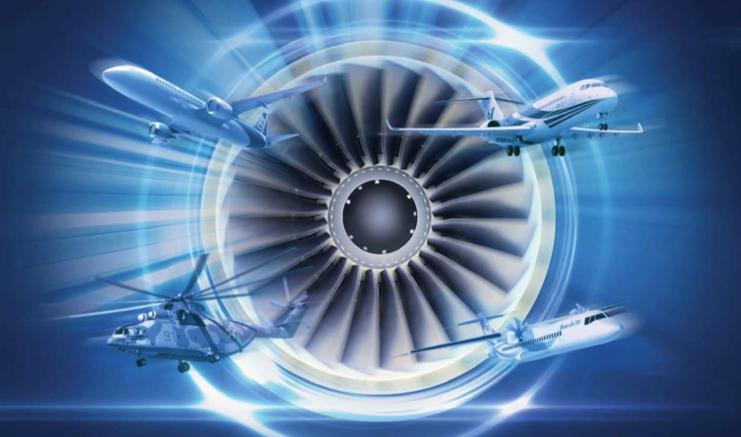
\includegraphics[scale=0.8]{1.png}
\\[1.5cm]
\HRule \\[0.3cm]
{ \huge \textsc{Tuyaux dynamique aérospatiale\\ }}\\[0.25cm] % Title of your document
\HRule \\[3cm]
 
\begin{minipage}{0.4\textwidth}
\begin{flushleft} \large
\emph{\textbf{Auteurs :}}\\

\textsc{De Leener} Maxime\\

\\[0,4cm]
\emph{\textbf{Cours :\ }}\\\textsc{\large LMECA 2830}\\[0.4cm] % Major heading such as course name


\end{flushleft}
\end{minipage}
~
\begin{minipage}{0.4\textwidth}
\begin{flushright} \large
%\emph{\textbf{Coordinateur :}} \\
% \textsc{}\\ [0,5cm] % Supervisor's Name

\emph{\textbf{Professeur :}} \\
\textsc{Chatelain} Philippe\\
\textsc{Schrooyen} Pierre\\ [0,4cm]

\emph{\textbf{Année académique :\ }}\\\textsc{\large 2017-2018}\\[0.4cm] % Minor heading such as course title
%\emph{\textbf{Date de remise :\ }}\\\textsc{\large \textcolor{red}{24 Mars 2017}}\\


\end{flushright}
\end{minipage}\\[0cm]


~
\begin{minipage}{0.4\textwidth}

\end{minipage}

\vfill % Fill the rest of the page with whitespace

\end{titlepage}

%\tableofcontents
\newpage


\chapter{Performance des avions}

\section{Convention de la mécanique du vol}
\subsection{L'atmosphère standard}

On utilise une atmosphère standard internationale (ISA) afin de comparer les performances de divers appareils dans des conditions atmosphériques semblables.

Elles sont les suivantes :
\begin{itemize}
    \item $R ~=~ 287,1~~[J/kgK]$ (air est un gaz parfait)
    \item l'air est sec
    \item le vent météorologique est nul (pas de turbulence atmosphériques)
    \item l’atmosphère est en équilibre hydrostatique, c’est-à-dire\\
    \begin{eqnarray}
    dp&=-\rho g(h) dh\\
    dp&=-\rho g_0 dH
    \end{eqnarray}
    avec $h$ l'altitude au-dessus du niveau de la mer et $H$ \textit{l'altitude géopotentielle} telle que $dH=\dfrac{g(h)}{g_0}dh$.
\end{itemize}

Avec l'équation d'état des gaz parfaits $p=\rho RT$, on obtient
\begin{eqnarray}
\dfrac{dp}{p}=-\dfrac{g_0}{RT(H)}dH
\end{eqnarray}

Aux latitudes moyennes (conditions tempérées), la distribution de température de l’atmosphère standard du niveau de la mer à une altitude de 20 km est la suivante :

\begin{eqnarray}
\textbf{Troposphère} &~~(0\le H\le 11~km)~&:~~T=288,16-6,5H\\
\textbf{Stratosphère} &~~(11~km\le H\le 20~km)~&:~~T=216,66
\end{eqnarray}

Cette distribution est représentée à la figure \ref{2}.

\begin{figure}[h!]
    \centering
    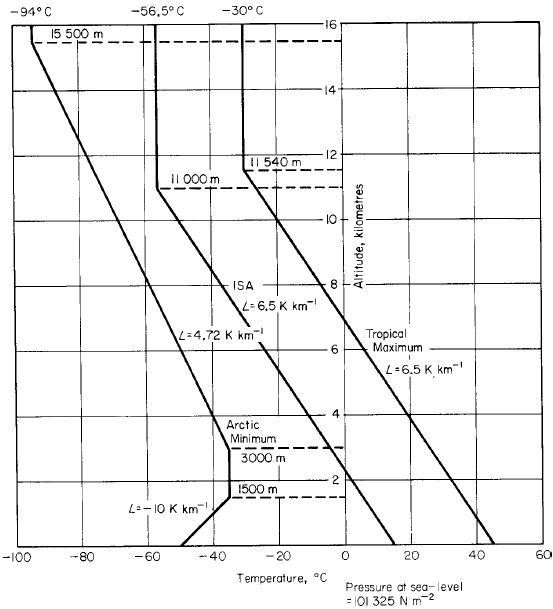
\includegraphics{2.JPG}
    \caption{Distribution de température en fonction de l’altitude dans l’atmosphère standard internationale}
    \label{2}
\end{figure}

\subsection{Altitude et vitesse de l'avion}
\subsubsection{L'altimètre}

La correspondance biunivoque entre altitude et pression dans l’atmosphère standard est mise à profit dans l’altimètre de l’avion, qui consiste en un manomètre (mesure de p) dont l’échelle est graduée en mètres (pieds) grâce à la relation entre pression et altitude. Contrairement aux manomètres de laboratoire qui sont généralement des manomètres à liquide (mercure, eau) et ne conviennent pas pour les avions, ce sont le plus souvent des manomètres à capsule (type Bourdon) dont la capsule est évacuée et qui se déforment en fonction de la pression extérieure. La déformation est communiquée à un système d’aiguille qui se déplace sur l’échelle. De nos jours, ces manomètres mécaniques sont de plus en plus souvent remplacés par des capteurs qui transforment la pression en signal électrique, mais les manomètres à capsule sont encore couramment
employés en aviation générale. Comme l’échelle est graduée à partir de l’atmosphère standard, le pilote doit effectuer les corrections en fonction des conditions atmosphériques locales. Sur les avions de ligne, ces données, communiquées par les tours de contrôle, sont intégrées par les ordinateurs de bord, qui effectuent automatiquement les corrections.

\subsubsection{L'indicateur de vitesse}


La vitesse de l'avion est déterminée à l'aide d'un tube pitot situé au nez de l'avion ou attaché à une aile. La différence de pression mesurée peut être reliée au nombre de Mach de vol (voir LMECA 2322).


\section{Vol en palier horizontal stabilisé}
\subsection{Équations d'équilibre}

La plupart des avions possèdent un plan de symétrie ce qui engendre que l'équilibre transversal est automatiquemet assuré. Il suffit donc d'étudier l'équilibre dans le plan de symétrie. 

\begin{figure}[h!]
    \centering
    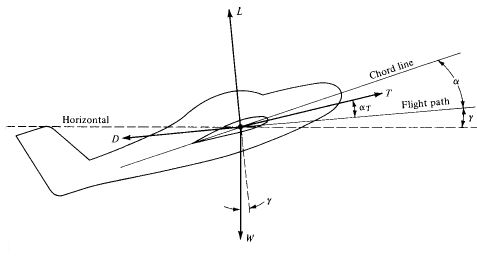
\includegraphics{3.JPG}
    \caption{Vol stabilisé - cas général}
    \label{3}
\end{figure}

Sur la figure \ref{3}, on peut apercevoir :
\begin{itemize}
    \item $\theta$ : l'angle d'assiette (entre l'axe de l'avion et l'horizontale géographique)
    \item $\alpha$ : l'angle d'incidence (entre la direction de la vitesse (vent) et l'axe de l'avion)
    \item $\gamma$ : la pente (entre la direction de la vitesse et l'horizontale géographique
\end{itemize}

On a donc \begin{eqnarray}
\theta ~=~ \gamma~+~\alpha
\end{eqnarray}

Il y a trois systèmes d'axes en mécanique du vol
\begin{itemize}
    \item \textit{Les axes aérodynamiques} (\textit{wind axes}) $x_a,~y_a,~z_a$ définis par l'alignement de $x_a$ avec le vecteur vitesse de l'avion
    \item \textit{les axes liés à l'avion} (\textit{body axes}) $x,~y,~z$
    \item \textit{les axes liés à la terre} (\textit{earth axes}) $x_0,~y_0,~z_0$ avec $z_0$ aligné avec l'accélération de la gravité.
\end{itemize}

Sur la figure \ref{3}, on a également $\alpha_T$ l'angle de la force de propulsion avec la direction de la vitesse. Donc $\epsilon = \alpha-\alpha_T$ (angle avec l'axe de l'avion).

\subsubsection{Équilibre selon $z_a$}

\begin{eqnarray}
W cos(\gamma)-L-Tsin(\alpha_T)=0
\end{eqnarray}

\subsubsection{Équilibre selon $x_a$}
\begin{eqnarray}
Tcos(\alpha_T)-D-W sin(\gamma)=0
\end{eqnarray}

Pour un vol horizontal à incidence modérée, ($\alpha_T<<1$), $T\approx D$. En configuration normale $D<<L$, de sorte que $Tsin(\alpha_T)<<L$. On obtient donc
\begin{eqnarray}
W&=&L\\
T&=&D
\end{eqnarray}

avec W, le poids de l'appareil.

La définition de la vitesse équivalente donne :
\begin{eqnarray}
V_E=\sqrt{\dfrac{2W}{\rho_s S C_L}} ~~\Leftrightarrow~~ C_L = \dfrac{2W}{\rho_s S V_E^2}
\end{eqnarray}

A faible nombre de Mach, $V_E\approx V_c$. $V_c$ est la la vitesse dite \textit{vitesse conventionnelle}.

Avec les coefficients aérodynamiques :
\begin{eqnarray}
C_L=\dfrac{L}{\bar{q}S} &~~~~~~&C_D=\dfrac{D}{\bar{q}S}
\end{eqnarray}

\subsection{Traînée et portance}

La traînée est représentée par $D$ pour \textit{drag} et la portance par $L$ pour \textit{lift}.

\begin{eqnarray}
D&= ~qSC_D&=~\dfrac{1}{2}\rho V^2 S C_D\\
L&= ~qSC_L &=~\dfrac{1}{2}\rho V^2 S C_L
\end{eqnarray}

\begin{figure}[h!]
    \centering
    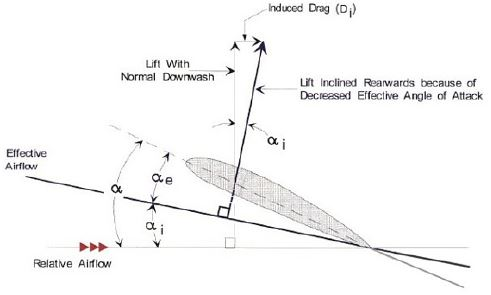
\includegraphics{4.JPG}
    \caption{Représentation de la traînée et de la portance}
    \label{4}
\end{figure}

\subsection{Poussée requise}

\begin{eqnarray}
\dfrac{T}{W}=\dfrac{C_D}{C_L}
\end{eqnarray}

$W$ est une donnée donc $T\propto\dfrac{C_D}{C_L}$.

\begin{figure}[h!]
    \centering
    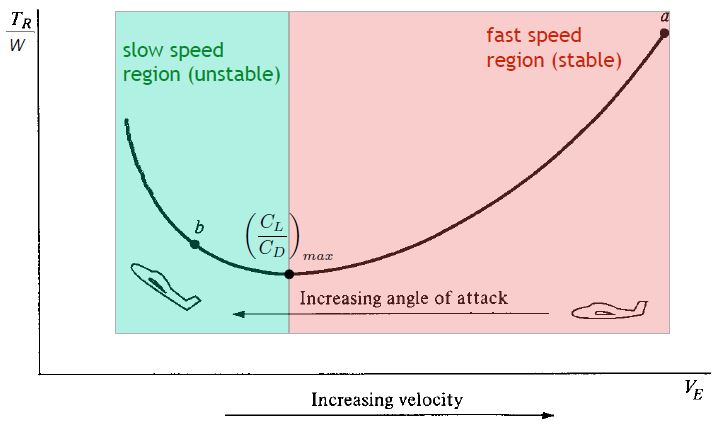
\includegraphics[scale=0.7]{5.JPG}
    \caption{Poussée requise au vol en palier}
    \label{5}
\end{figure}

On peut s'apercevoir, sur la figure \ref{5}, que pour une poussée $T$ donnée, il existe deux configurations de vol possibles. Le \textit{régime lent} et le \textit{régime rapide}. Il existe également une vitesse équivalente particulière pour laquelle la poussée requise est minimale.

La polaire des avions est de la forme :
\begin{eqnarray}
C_D &= &C_{D,e}+\dfrac{C_L^2}{\pi e AR}\\
C_D &= &C_{D,0}+\dfrac{C_L^2}{\pi e^* AR}\\
C_D &= &C_{D,0}+kC_L^2\\
\end{eqnarray}

avec 
\begin{itemize}
    \item $C_{D,e}$ la traînée parasite qui contient encore la composante de portance.
    \item $AR=\dfrac{b^2}{S}$, le ratio d'aspect (aspect ratio)
    \item $e$ le rendement de l'envergure (span efficiency)
    \item $e^*$ le rendement d'Oswald (Oswald efficiency)
    \item $C_{D,0}$ la traînée dite parasite, essentiellement visqueuse. 
    \item $kC_L^2$ la traînée de portance.
\end{itemize}

On peut donc réexprimer $\dfrac{T}{W}$ :
\begin{eqnarray}
\dfrac{T}{W} &= &C_{D,0}+kC_L^2\\
 &= &\dfrac{C_{D,0}}{C_L(V_E)}+kC_L(V_E)\\
T  &= &qSC_{D,0}+\dfrac{kW^2}{qS}
\end{eqnarray}


\textbf{Note :} $T=\dfrac{W}{C_L/C_D}$ ($T_{min}$ quand $\dfrac{C_L}{C_D}$ est maximum).

On peut déterminer analytiquement le $C_L$ correspondant à la traînée minimum et donc à la poussée requise minimum :

\begin{eqnarray}
\dfrac{d(C_D/C_L)}{dC_L} &= &-\dfrac{C_{D,0}}{C_L^2}+k=0\\
C_{L,T_{min}} &= &\sqrt{\dfrac{C_{D,0}}{k}}\\
C_{D,T_{min}} &= &2C_{D,0}\\
\left.\dfrac{C_D}{C_L}\right|_min &= &\sqrt{4kC_{D,0}}
\end{eqnarray}

Remarquez que la configuration de traînée minimale correspond à l’égalité de la traînée parasite et de la traînée de portance.

\begin{figure}[h!]
    \centering
    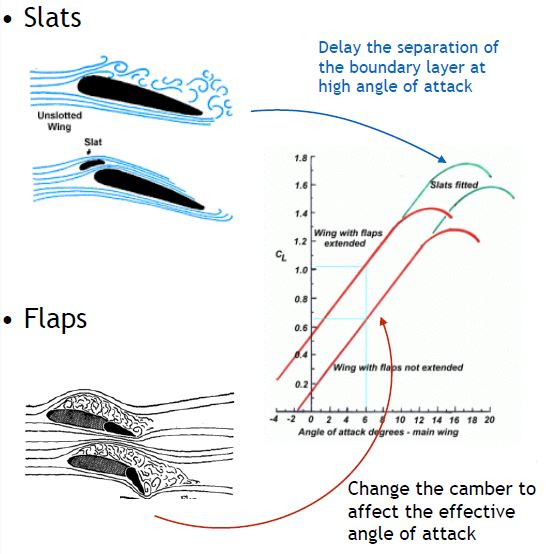
\includegraphics[scale=0.7]{6.JPG}
    \caption{Influence des flaps et slats}
    \label{6}
\end{figure}

\subsection{Poussée requise pour un vol en palier non-accéléré}

\subsubsection{Thrust}
\begin{figure}[h!]
    \centering
    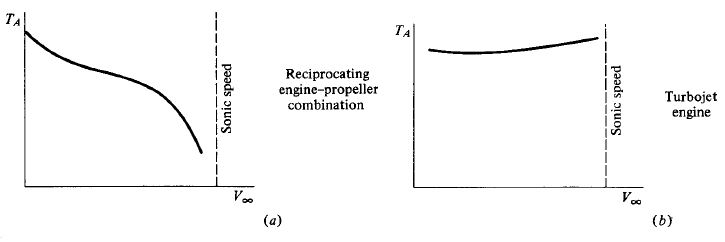
\includegraphics[scale=0.7]{7.JPG}
    \caption{Courbes de poussée disponible pour les hélices entraînées par moteur à piston et pour les turboréacteurs}
    \label{7}
\end{figure}

A chaque altitude, on peut déterminer une vitesse équivalente maximum et minimum (le plus souvent fixée par la limite de décrochage) et on peut calculer les vitesses vraies correspondantes. Ceci définit dans le plan H,V une courbe appelée l’enveloppe de vol stabilisé et qui contient le domaine de vol. On observe sur l’enveloppe de vol l’avantage de voler en altitude : la vitesse maximale est atteinte en altitude, pour une poussée et donc une consommation plus faible.

\begin{figure}[h!]
    \centering
    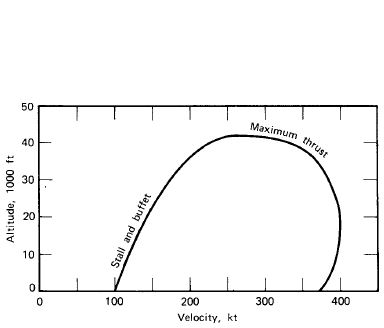
\includegraphics{8.JPG}
    \caption{Enveloppe de vol typique}
    \label{8}
\end{figure}

\paragraph{Stabilité de propulsion} Supposons que l'avion subisse une perturbation de vitesse $\Delta V$.
\begin{itemize}
    \item \textbf{Régime rapide}  Si $\Delta V>0$, on voit que $C_D/C_L$ augmente, alors que $T/W$ reste constant. L'avion a donc tendance à ralentir, le régime de vol est statiquemet stable.
    \item \textbf{Régime lent}  En eVectuant le même raisonnement, on constate que le régime lent est statiquement instable. C’est donc un régime dangereux, qu’il convient d’éviter, particulièrement lors des phases de décollage ou d’atterrissage. En effet, si la vitesse tombe sous la vitesse de poussée requise minimale, il n’est pas toujours possible d’augmenter la poussée (en poussant la manette) suffisamment ou assez vite pour éviter le décrochage. On pourrait penser que cette limitation est plus restrictive que la limitation liée au décrochage mais à l’atterrissage, en raison du déploiement des spoilers, volets et train d’atterrissage, le$C{D,0}$ augmente brutalement, ce qui déplace le $C{L,T}$ min vers le haut et élargit donc la zone de régime rapide vers les basses vitesses.
\end{itemize}

\subsection{Puissance requise pour un vol en palier non-accéléré}

\begin{eqnarray}
P_R &= &T_RV_\infty =\dfrac{W}{C_L/C_D}V_\infty = \dfrac{W}{C_L/C_D}\sqrt{\dfrac{2W}{\rho_s C_L S}}\\
P_R &= &\sqrt{\dfrac{2W^3C_D^2}{\rho_s S C_L^3}}\propto \dfrac{C_D}{C_L^{3/2}}\\
& = &W^{3/2}\sqrt{\dfrac{2}{\rho_s S}}\dfrac{C_{D,0}+kC_L^2}{C_L^{3/2}}
\end{eqnarray}

Calculons, pour une altitude donnée, la puissance minimum requise au vol.

\begin{eqnarray}
\dfrac{d(C_D/C_L^{3/2})}{dC_L} &= &-\dfrac{3}{2}\dfrac{C_{D,0}}{C_L^{5/2}}+\dfrac{1}{2}\dfrac{k}{C_L^{1/2}}=0\\
C_{L,P_{R,min}} &= &\sqrt{\dfrac{3C_{D,0}}{k}}\\
C_{D,P_{R,min}} &= &4C_{D,0}\\
\left.\dfrac{C_D}{C_L^{3/2}}\right|_{min} &= &\dfrac{4C_{D,0}}{(3C_{D,0}/k)^{3/4}}
\end{eqnarray}

On constate que $C_{L,P_{R,min}}>C_{L,T_{min}}$ et donc que $V_{E,P_{R,min}}<V_{E,T_{min}}$

\textbf{Note :} La puissance disponible $P_a$ est : 
\begin{eqnarray}
P_a=P_{a,s} \dfrac{\rho}{\rho_s}
\end{eqnarray}

Avec $s$ qui signifie "au niveau de la mer".

\begin{figure}[h!]
    \centering
    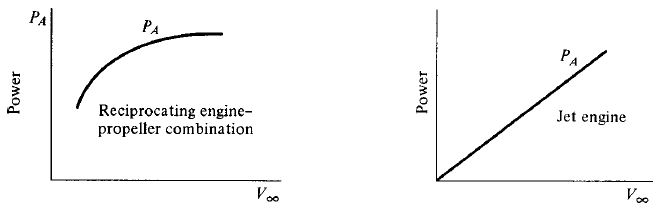
\includegraphics[scale=0.7]{9.JPG}
    \caption{Courbes de puissance disponible pour les hélices entraînées par moteur
à piston et pour les turboréacteurs}
    \label{9}
\end{figure}

\begin{figure}[h!]
    \centering
    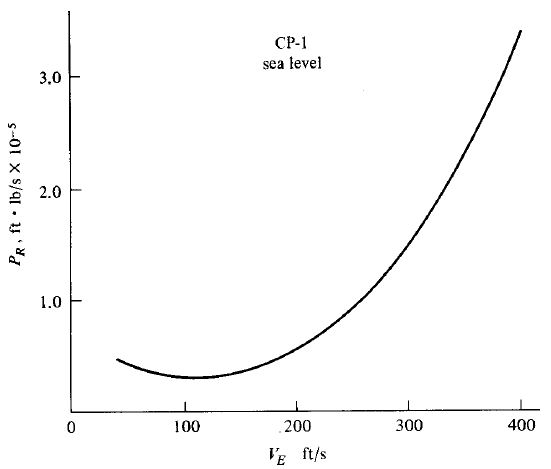
\includegraphics[scale=0.8]{10.JPG}
    \caption{Puissance requise au vol en palier}
    \label{10}
\end{figure}

\textbf{Note :} Pour les avions à hélice, on peut faire les observations suivantes :
\begin{itemize}
    \item Du fait que $V_{E,W_{min}}<V_{E,T_{min}}$ et que d'autre part la puissance disponible ne croît que légèrement avec la vitesse pour les avions à hélice (voir figure \ref{9}), il n'y a quasiment pas de régime lent pour ces appareils. Il y a donc peu de risques d'instabilités de propulsion.
    \item Du fait que la puissance disponible est approximativement proportionnelle à la masse volumique, $W_{disp}\sqrt{\sigma}\propto\sigma^{3/2}$ décroît rapidement avec l’altitude. Il en résulte que le plafond est généralement plus faible pour les avions à hélice que pour les avions à réaction. En outre, l’enveloppe de vol est moins penchée vers les hautes vitesses comme illustré ci-dessous (figure \ref{11}) pour le Cherokee Arrow\footnote{Noter la limite de décrochage qui apparaît très clairement}. Il est donc moins intéressant de voler en altitude.
\end{itemize}

\begin{figure}[h!]
    \centering
    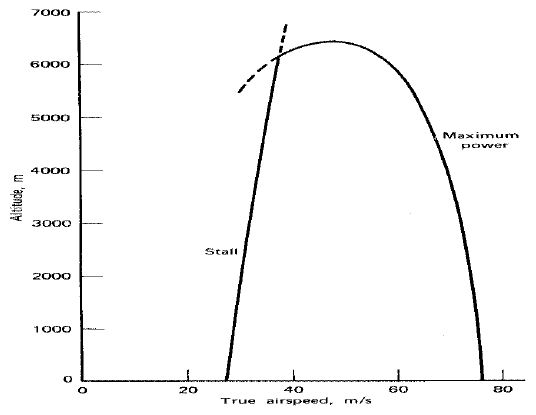
\includegraphics[scale=0.8]{11.JPG}
    \caption{Enveloppe de vol pour le Cherokee Arrow}
    \label{11}
\end{figure}

\subsection{Distance franchissable (Range)}

\subsubsection{Définition} La connaissance du vol en palier horizontal stabilisé va nous permettre de calculer approximativement la distance franchissable ou encore rayon d’action de l’avion. Il existe trois définitions du rayon d’action.

\paragraph{Rayon d’action de sécurité} Distance horizontale maximum entre deux aéroports
que peut parcourir un avion de manière sécuritaire en effectuant un service
régulier et fiable. Pour calculer ce rayon d’action, il faut tenir compte d'énormément de facteurs comme 
\begin{itemize}
    \item carburant consommé au décollage,
    \item montée initiale/descente finale,
    \item règles de sécurité qui exigent de conserver à toutmoment suYsamment
de carburant pour pouvoir se détourner,
\item conditions météo défavorables (vent de face),
\item ...
\end{itemize}
Ceci rend le calcul extrêmement long et complexe. C’est pourquoi on utilise
également deux définitions simples mais nécessairement plus artificielles,
qui sont surtout utiles pour comparer deux appareils entre eux.

\paragraph{Rayon d’action SAR (still air range)} On suppose que l’avion décolle réservoir
plein, rejoint ses conditions de vol de croisière (altitude, vitesse) et poursuit
son vol jusqu’à épuisement du carburant. Le SAR est la distance franchie,
à l’exclusion du décollage.

\paragraph{Rayon d’action GSAR (gross still air range)} On considère un scénario encore plus
simple : soit l’avion initialement dans les conditions de vol de croisière, réservoirs
pleins. Le GSAR est la distance qu’il franchirait en palier jusqu’à
épuisement du carburant. Ce concept est évidemment extrêmement artificiel
mais il offre l’avantage d’être très simple à calculer et de fournir les
tendances du rayon d’action avec divers paramètres.

\subsubsection{Calcul du rayon d'action pour un avion à réaction}

Pour un avion à réaction, on définit la consommation spécifique comme
\begin{eqnarray}
c = \dfrac{\dot{m_c}}{T}=\dfrac{\text{débit de carburant}}{\text{poussée}}~~[\frac{kg/s}{N}]
\end{eqnarray}

\textbf{Note :} $c$ est aussi appelée $TSFC$ (Thrust Specific Fuel Consumption) dans le cours.

\begin{eqnarray}
\dfrac{dW}{dt} = -gcT
\end{eqnarray}

Or, en palier, $T=W(C_D/C_L)$. Donc,
\begin{eqnarray}
\dfrac{dW}{dt} = -\dfrac{gcC_D}{C_L}W & \text{ou encore} & dt=-\dfrac{C_L}{gcC_D}\dfrac{dW}{W}
\end{eqnarray}

La distance parcourue par l'avion en $dt$ est $dx=Vdt$, d'où
\begin{eqnarray}
dx = -\dfrac{V}{gc}\dfrac{C_L}{C_D}\dfrac{dW}{W} = -\dfrac{C_L}{C_D}\dfrac{V}{c W}dm
\end{eqnarray}
pour un avion à réaction.

\paragraph{Specific air range (SAR)}: distance parcourue en brûlant une unité de masse de carburant 
\begin{eqnarray}
SAR = \dfrac{C_L V}{cC_DW}~~[\frac{m}{kg}]
\end{eqnarray}

\paragraph{Le rayon spécifique unitaire (USAR)}: distance parcourue en brûlant une unité de masse de carburant par unité de masse de l’avion
\begin{eqnarray}
USAR = \dfrac{C_L V}{gcC_D}~~[m]
\end{eqnarray}

We can integrate this with assumptions :
\begin{eqnarray}
V=\sqrt{\dfrac{2W}{\rho C_L S}} 
\end{eqnarray}

donc soit :
\begin{itemize}
    \item $C_L,~V$ = constantes
    \item $C_L,~\rho$ (altitude) = constantes
    \item $V,~\rho$ = constantes
\end{itemize}


On obtient la formule de Bréguet-Leduc (Gross Specific Air Range for jets)
\begin{eqnarray}
GSAR &= \dfrac{C_L}{C_D}\dfrac{V}{c g} ln(\dfrac{W_1}{W_2})\\
GSAR &= USAR ln(\dfrac{W_1}{W_2})
\end{eqnarray}

Avec $W_1$ le poids initial de l'avion et $W_2$ le poids après épuisement du carburant

\subsubsection{Calcul du rayon d'action pour un avion à hélice}

Pour un avion à hélice, on utilise la notion d’efficacité du moteur plutôt que la notion de consommation spécifique, à savoir
\begin{eqnarray}
\eta_m = \dfrac{P_m}{q_c L}=\dfrac{\text{Puissance}~[W]}{\text{débit de carburant}~[kg/s]~~\text{pouvoir calorifique}~~[J/kg]}
\end{eqnarray}
car $\eta_m$ dépend peu de la vitesse, On peut alors écrire
\begin{eqnarray}
g q_c = -\dfrac{dW}{dt}=g\dfrac{W_m}{\eta_m L}
\end{eqnarray}

Le rendement de propulsion $\eta_p$ étant lui défini comme le rapport entre la puissance propulsive $w=TV$ et la puissance mécanique à l'arbre du moteur $W_m$, on en déduit
\begin{eqnarray}
\dfrac{dW}{dt}=-g\dfrac{TV}{\eta_p\eta_m L}=-\dfrac{gP}{\eta L}\dfrac{C_D}{C_L}V
\end{eqnarray}

et donc
\begin{eqnarray}
dx=-\dfrac{\eta L}{g}\dfrac{C_L}{C_D}\dfrac{dW}{W} = -\dfrac{\eta}{gSFC}\dfrac{C_L}{C_D}\dfrac{dW}{W} \\
USAR = \dfrac{\eta L}{g}\dfrac{C_L}{C_D}
\end{eqnarray}

En intégrant :

\begin{eqnarray}
R= \dfrac{\eta_p}{SFC}\dfrac{C_L}{C_D g}ln(\dfrac{W_1}{W_2})=USAR ln(\dfrac{W_1}{W_2})
\end{eqnarray}

\textbf{Note :}
avec SFC (specific fuel consumption) : $SFC=\frac{q_c}{P}=\frac{\text{fuel consumption}}{power}$
\begin{eqnarray}
P_A &= &\eta P\\
P &= &\dfrac{TV}{\eta_T}\\
\dfrac{T}{W} &= &\dfrac{D}{L}\\
\dfrac{dW}{dt} &= &-SFC g P\\
\dfrac{dW}{dt} &= &-g SFC \dfrac{W C_D V}{\eta_p C_L}
\end{eqnarray}

\subsubsection{Optimisation du rayon d'action}

\paragraph{Avion à réaction} Il faut maximiser le rapport $VC_L/C_D$. Or, parmis les trois variables $\rho,~V,~C_L$, deux sont indépendantes. Le problème d'optimisation dépendra donc de la contrainte (relation entre les variables indépendantes) imposée.
\begin{enumerate}
    \item Optimisation à $\rho$ imposé\\
    \begin{eqnarray}
    \dfrac{d}{dC_L}\left(\dfrac{V C_L}{C_D}\right)_\rho=0
    \end{eqnarray}
    On sait que
    \begin{eqnarray}
    \dfrac{VC_L}{C_D}\propto \dfrac{C_L^{1/2}}{C_D}
    \end{eqnarray}
    Avec la polaire parabolique, on obtient alors un optimum pour
    \begin{eqnarray}
    \left. C_L\right|_{rao}=\sqrt{\dfrac{C_{D,0}}{3k}}&\rightarrow & V_{rao}=\sqrt{\dfrac{2W}{\rho S}}\left(\dfrac{3k}{C_{D,0}}\right)^{1/4}
    \end{eqnarray}
    
    \item Optimisation à position de la manette des gaz imposée\\
    Cela impose :
    \begin{eqnarray}
    T(\rho,\Pi)=\rho\dfrac{V^2}{2}SC_D
    \end{eqnarray}
    avec $\Pi$ la position de la manette des gaz. A $\Pi$ donnée, on suppose la poussée $T$ proportionnelle à $\rho$ :
    \begin{eqnarray}
    T_0(\Pi)=\rho_0\dfrac{V^2}{2}SC_D~~\rightarrow~~V\propto C_D^{-1/2}~~\rightarrow~~\dfrac{VC_L}{C_D}\propto\dfrac{C_L}{C_D^{3/2}}
    \end{eqnarray}
    Avec la polaire parabolique, on obtient alors un optimum pour
    \begin{eqnarray}
    \left. C_L\right|_{rao}=\sqrt{\dfrac{C_{D,0}}{2k}}&\rightarrow & V_{rao}=\sqrt{\dfrac{2W}{\rho S}}\left(\dfrac{2k}{C_{D,0}}\right)^{1/4}
    \end{eqnarray}
    L'altitude correspondante à l'optimum résulte alors de l'équation de sustentation
    \begin{eqnarray}
    \rho = \dfrac{2W}{V^2SC_L}
    \end{eqnarray}
    
    \item Optimisation à V imposée\\
    Dans ce cas, la solution est élémentaire, l’optimum est atteint pour l’incidence de finesse maximum. Dans ce cas également, $\rho$ est déduit de l’équilibre en sustentation.
\end{enumerate}

\textbf{Note :} Parmis les 3 optimisation, c'est certainement la première qui a le plus de signification pratique.\\
\begin{eqnarray}
GSAR_{opt} = \dfrac{C_L V_{rao}}{gcC_D}ln\dfrac{W_1}{W_2}
\end{eqnarray}

Etant donné que $V_{rao}\propto\sqrt{\frac{P}{S}}$, il apparaît que le rayon d'action est fonction croissante de la charge alaire $P/S$ (que l'on augmente en réduisant la surface alaire et non en augmentant le poids!). L'augmentation du rayon d'action est donc en contradiction avec la réduction de la vitesse d'atterrissage/décollage. Enfin, comme $V_{rao}\propto(\frac{k}{C_{D,0}})^{1/4}$ mais que par ailleurs, $(C_L/C_D)_{rao}\propto (kC_{D,0})^{-1/2}$, on augmente le rayon d'action en réduisant k (càd en aumentant l'allongement) mais surtout $C_{D,0}$.

\paragraph{Avion à hélice} Dans le cas de l’avion à hélice, la vitesse n’intervenant pas dans l’expression du USAR, le rayon d’action maximum s’obtient en maximisant la finesse $C_L/C_D$, quelle que soit la contrainte imposée (altitude, position de la manette des gaz ou vitesse).

\subsection{Endurance}

L’endurance est le temps de vol correspondant au rayon d’action GSAR. 

\subsubsection{Avion à réaction}
\begin{eqnarray}
\dfrac{dP}{dt}=-gcE=-g\cdot TSFC\cdot E\\
E=\dfrac{C_L}{g\cdot TSFC\cdot C_D}ln(\dfrac{W_1}{W_2})
\end{eqnarray}
et l’on voit que l’endurance est optimisée à l’incidence de finesse maximum.

\subsubsection{Avion à hélice}

\begin{eqnarray}
\dfrac{dP}{dt}=-\dfrac{gP}{\eta L}\dfrac{C_D}{C_L}V~~\rightarrow~~dt=-\dfrac{\eta L}{g}\dfrac{C_L}{VC_D}\dfrac{dP}{P}\\
E=\dfrac{\eta_p}{gSFC}\dfrac{C_L^{3/2}}{C_D}\sqrt{2\rho S}(W_1^{-1/2}-W_0^{-1/2})
\end{eqnarray}

L'endurance est donc optimisée en maximisant $\dfrac{\eta L}{g}\dfrac{C_L}{VC_D}$

\section{Vol stabilisé incliné (montée/descente)}
\subsection{Conséquence des équations d'équilibre}

On peut simplifier les équations d'équilibre :
\begin{eqnarray}
W cos(\gamma)-L=0\\
T-D-W sin(\gamma)=0
\end{eqnarray}

On a V=cste et $\gamma$=cste. Comme
\begin{eqnarray}
W cos(\gamma)=L=\rho\dfrac{V^2}{2}SC_L
\end{eqnarray}

Il en résulte que $\rho C_L$ doit rester constant (ignorant variation de masse due à la conso de carburant).

D'autre part, l'équation de propulsion donne
\begin{eqnarray}
T=W sin(\gamma)+\dfrac{C_D}{C_L}L=W sin(\gamma)+\dfrac{C_D}{C_L}Wcos(\gamma)
\end{eqnarray}

\begin{eqnarray}
\text{sustentation} & Wcos(\gamma)-L=\dfrac{W V^2}{gR}=\dfrac{W}{g}V\omega = -\dfrac{W}{g}V\dfrac{d\gamma}{dt}\\
\text{propulsion} & T-D-W sin(\gamma) = \dfrac{W}{g}\dfrac{dV}{dt}
\end{eqnarray}

\subsection{Cas particulier : le vol plané}

Dans ce cas, il n'y a pas de poussée : $T=0$. On a donc $L<W$.

\begin{figure}[h!]
    \centering
    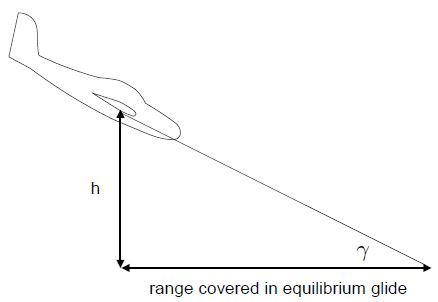
\includegraphics[scale=0.7]{12.JPG}
    \caption{Avion entrain de planer}
    \label{12}
\end{figure}

\begin{eqnarray}
tan(\gamma) = -\dfrac{D}{L}=-\dfrac{C_D}{C_L}\\
Range_{gliding}=\int_H^0\dfrac{dH}{tan(\gamma)}
\end{eqnarray}

Pour maximiser la distance parcourue, il faut minimiser $|tan(\gamma)|$. Ceci est obtenu à l'incidence de finesse maximum, et que la pente minimum est indépendante de l'altitude et du poids de l'avion.

On peut également calculer la vitesse de descente $w_d$ :

\begin{eqnarray}
w_d=\dfrac{R}{D}=\sqrt{\dfrac{2W}{\rho S}}cos^{\frac{3}{2}}(\gamma)\dfrac{C_D}{C_L^{\frac{3}{2}}}
\end{eqnarray}

\subsection{Vol motorisé : vitesse ascensionnelle maximum}

\begin{eqnarray}
\dfrac{R}{C}=V_\infty sin(\gamma)\\
\dfrac{T-D}{W}=sin(\gamma)\\
\dfrac{R}{C}=\dfrac{TV-DV}{W}=\dfrac{\text{Power Available}-\text{Power required}}{W}\\
W cos(\gamma)-L=0\\
\end{eqnarray}

La vitesse ascensionnelle :
\begin{eqnarray}
w_a=V sin(\gamma)
\end{eqnarray}

\begin{figure}[h!]
    \centering
    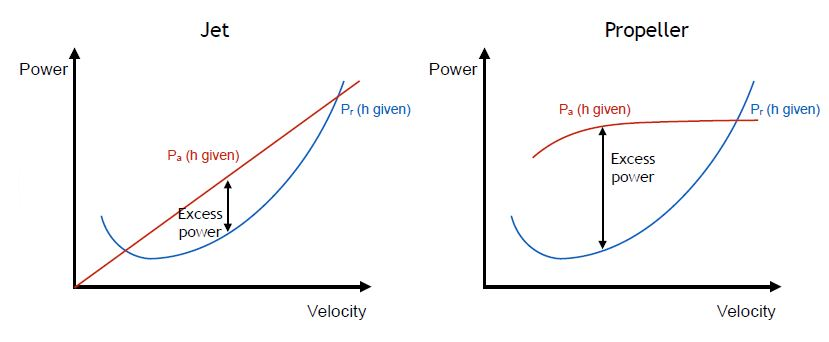
\includegraphics[scale=0.7]{13.JPG}
    \caption{Puissance en fonction de la vitesse}
    \label{13}
\end{figure}

\subsubsection{Point de vue de l'avion à réaction}

Nous voulons déterminer dans quelles conditions d'incidence on pourra obtenir une vitesse ascensionnelle maximum avec un avion à réaction (T indépendant de V).

Avec un faible angle de montée ($cos(\gamma)\approx 1$ et $L\approx P$,
\begin{eqnarray}
sin(\gamma) = \dfrac{T-D}{P}=\frac{T}{P}-\frac{C_D}{C_L}
\end{eqnarray}

L'angle de montée max est obtenu à incidence de finesse max. Si on multiplie par $V$ :
\begin{eqnarray}
w_a = \sqrt{\dfrac{2Wcos(\gamma)}{\rho SC_L}}\left(\dfrac{T}{p}-\dfrac{C_D}{C_L}\right)
\end{eqnarray}

Pour maximiser la vitesse ascensionnelle, il faut donc maximiser le produit $\xi =C_L^{-1/2}(T/P-C_D/C_L)$.
\begin{eqnarray}
\dfrac{d\xi}{dC_L}=-\dfrac{1}{2}C_L^{-3/2}\dfrac{T}{W}+\dfrac{3}{2}C_L^{-5/2}C_{D,0}-\dfrac{1}{2}C_L^{-1/2}k=0
\end{eqnarray}

On sait que $C_D=C_{D,0}+kC_L^2$, on arrive donc à
\begin{eqnarray}
kC_L^2+C_L\dfrac{T}{W}-3C_{D,0}=0
\end{eqnarray}

Cette équation est assez simple à résoudre, remarquons que $T/P$ varie avec l'altitude, la vitesse ascensionnelle maximum sera atteinte pour des incidences qui varieront donc avec l'altitude.

\subsubsection{Point de vue de l'avion à hélice}

Lorsque l'angle de montée est faible ($<13\degree$), les changements de portance, traînée et vitesse causées par l'inclinaison de la trajectoire peuvent être négligés. Dès lors, la puissance requise pour vaincre la traînée diffère un peu de celle du vol horizontal dans les mêmes conditions d'altitude et de vitesse (c-à-d d'incidence). Dans ces conditions, si dans une configuration de vol donnée, on dispose d'un excès de puissance $\Delta P$, celui-ci provoquera une vitesse ascensionnelle $w_a$ telle que $w_aW=\Delta P$, ce que l'on voit immédiatement avec :
\begin{eqnarray}
w_a = Vsin(\gamma)=V\dfrac{T-D}{W}=\dfrac{P_{disp}-P_{req}}{W}=\dfrac{\Delta P}{W}
\end{eqnarray}

On a \begin{eqnarray}
\dfrac{\delta P_R}{\delta V_E}=0 ~~\Rightarrow~~C_{L,P_{max}}=\sqrt{\dfrac{3C_{D,0}}{k}}
\end{eqnarray}

\section{Manoeuvres}

\subsection{Décollage}

\begin{figure}[h!]
    \centering
    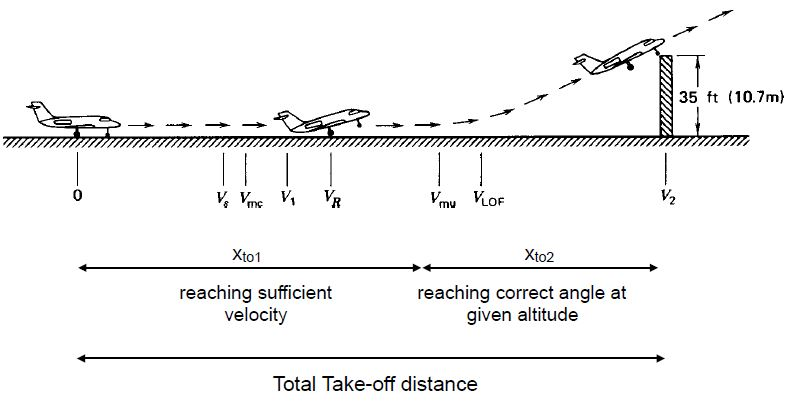
\includegraphics[scale=0.7]{14.JPG}
    \caption{Schéma de la manoeuvre de décollage selon la norme FAR Part 25 (aviation de ligne)}
    \label{14}
\end{figure}

L'équation du mouvement est simple :

\begin{eqnarray}
m\frac{dv}{dt} = T-D-\mu_T (W-L)
\end{eqnarray}

avec $(W-L)$ la force net appliquée aux roues, $\mu_T$ le facteur de frottement sur la piste ($\approx 0,02$ pour de l'asphalte et $\approx0,1$ pour de la pelouse).

Négligeons la traînée et les frottements de roulement ($D-\mu_T(W-L)$ négligé) :
\begin{eqnarray}
\dfrac{W}{g}\dfrac{dV}{dt}&=T\\
V&=\dfrac{dx}{dt}\\
x_{to}&=\dfrac{W}{Tg}\dfrac{V_{to}^2}{2}
\end{eqnarray}

La vitesse de décrochage est :
\begin{eqnarray}
V_s=\sqrt{\dfrac{2W}{\rho S C_{L,max}}}
\end{eqnarray}

Et on définit la vitesse de décollage comme :
\begin{eqnarray}
V_{to}=1,2V_s
\end{eqnarray}

On a donc 
\begin{eqnarray}
x_{to} &= \dfrac{W}{Tg}\dfrac{2W}{\rho_sC_{L,max} 2S}(1,2)^2 = \dfrac{1,44 W^2}{T g \rho C_{L,max} S}\\
x_{to} &= \dfrac{1,44 W^2}{g\rho S C_{L,max}(T-(D+\mu(W-L)))} 
\end{eqnarray}

\textbf{Note :}\begin{itemize}
    \item la distance au sol est extrêmement sensible au poids, variant quadratiquement avec celui-ci,
    \item la distance au sol dépend fortement des conditions atmosphériques locales, étant inversément proportionnelle au carré de la masse volumique,
    \item la distance au sol diminue en augmentant la surface alaire, le $C_{L,max}$ et la poussée. Comme on l'a mentionné précédemment, l'augmentation de la surface alaire influence cependant négativement la distance franchissable. C'est également le cas de l'augmentation de la poussée car elle ne peut s'obtenir que par l'installation d'un moteur plus lourd.
\end{itemize}

Si on prend la traînée et le frottement au roulement en compte, 
\begin{eqnarray}
D=\frac{1}{2}\rho S V^2 \left(C_{D,0}+\dfrac{\phi C_L^2}{\pi e^* AR}\right)
\end{eqnarray}

avec
\begin{eqnarray}
\phi = \dfrac{(16h/b)^2}{1+(16h/b)^2}
\end{eqnarray}

où $h$ est la hauteur de l'aile, $b$ son envergure et $\phi$ est l'effet de sol (diminution de traînée induite).

Pour des calculs préliminaires, on préfère souvent utiliser le modèle simplifié suivant : on approxime la trajectoire de l’avion lors de cette phase d’arrondi par un arc de cercle. Dès lors, les hauteur et pente en fin d’arrondi étant respectivement h et $\gamma$, la distance parcourue du point de décollage à la fin de l’arrondi est

\begin{eqnarray}
x_{to,2} \approx 2\dfrac{h}{tan(\gamma)}
\end{eqnarray}

La hauteur h est prise égale à 35 pieds et la pente est calculée en considérant un vol incliné stabilisé, de sorte que

\begin{eqnarray}
tan \gamma\approx sin\gamma = \dfrac{T-D}{W}\approx\dfrac{T}{W}-\dfrac{C_D}{C_L}
\end{eqnarray}


\subsection{Atterrissage}

\begin{figure}[h!]
    \centering
    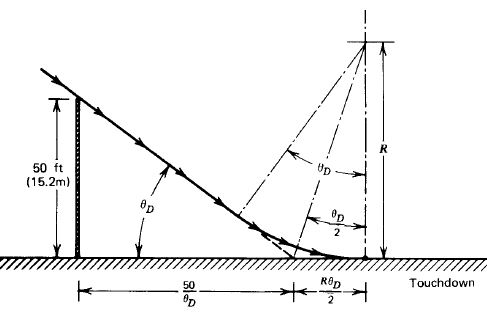
\includegraphics{15.JPG}
    \caption{Schéma de la manoeuvre d'atterrissage composée de \textit{l'approche}, \textit{l'arrondi} et \textit{le freinage au sol}}
    \label{15}
\end{figure}

La vitesse de décrochage est sensiblement plus faible qu'au décollage car le coefficient de portance maximum est supérieur mais aussi d'une charge alaire plus faible.

\begin{eqnarray}
V_{s,att} = \sqrt{\dfrac{2W}{\rho SC_{L,max}}}
\end{eqnarray}

Si on dénote par R le rayon de courbure de l'arrondi, la distance parcourue en l'air est
\begin{eqnarray}
s_2=\frac{h}{tan(\gamma)}+T tan\left(\dfrac{\gamma}{2}\right)
\end{eqnarray}

\subsection{Vol tournant}
\subsubsection{La ressource}
Rotation dans le plan de symétrie de l'avion (inclinaison du nez).

\begin{figure}[h!]
    \centering
    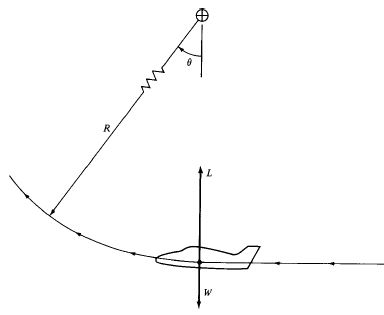
\includegraphics{16.JPG}
    \caption{Schéma de la ressource}
    \label{fig:my_label}
\end{figure}

Les équations du mouvement lors de la manoeuvre sont :
\begin{eqnarray}
W cos(\gamma)-L=\dfrac{WV^2}{gR}~~(\text{sustentation})\\
T-D-W sin(\gamma)=0~~(\text{propulsion})
\end{eqnarray}

Au point bas de la ressource ($\gamma=0$), on obtient
\begin{eqnarray}
W-L=\dfrac{W V^2}{gR}\\
T=D
\end{eqnarray}

On définit un facteur de charge de la manoeuvre, noté n comme le rapport entre la portance et le poid :
\begin{eqnarray}
n\triangleq \dfrac{L}{W}
\end{eqnarray}

Dans ce cas
\begin{eqnarray}
n=\left(1+\dfrac{V^2}{gR}\right)
\end{eqnarray}

\subsection{Vol en virage}

\begin{figure}[h!]
    \centering
    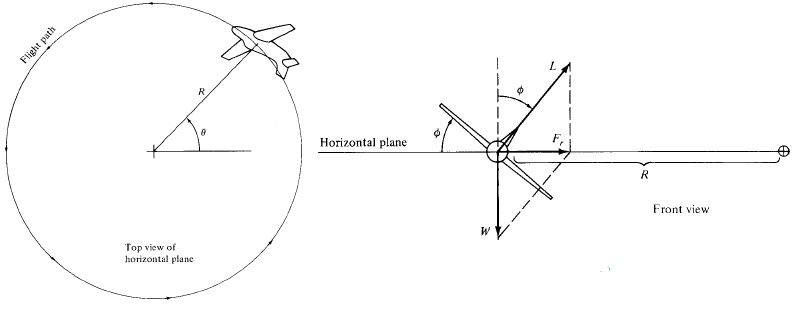
\includegraphics[scale=0.75]{17.JPG}
    \caption{Avion en virage horizontal}
    \label{17}
\end{figure}

\chapter{Stabilité statique et guidage}

\begin{figure}[h!]
    \centering
    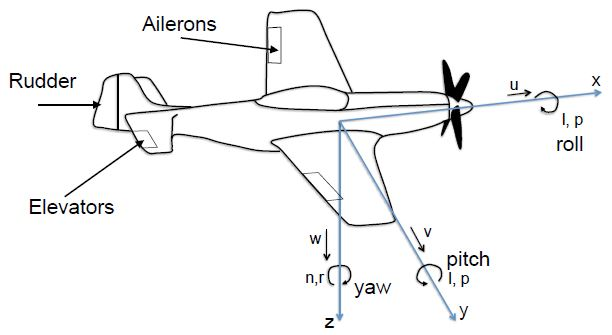
\includegraphics[scale=0.7]{18.JPG}
    \caption{Rotations et axes de l'avion}
    \label{18}
\end{figure}

\paragraph{Stabilité statique} étude de la tendance initiale d'un véhicule à retourner à son point d'équilibre après perturbation.

\paragraph{Stabilité dynamique} étude de l'historique temporel de la réponse à une perturbation.

\paragraph{Contrôle} étude du changement d'une configuration à une autre de l'avion.

\section{Stabilité statique longitudinale - manche fixe}

\begin{figure}[h!]
    \centering
    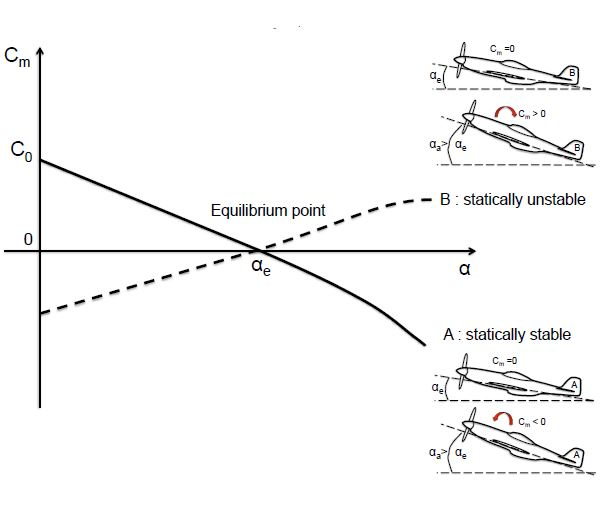
\includegraphics[scale=0.7]{19.JPG}
    \caption{Moment de tangage en fonction de l'incidence}
    \label{19}
\end{figure}

\subsection{Stabilité statique}

Il faut que 
\begin{eqnarray}
C_{m0} &> &0\\
\dfrac{\partial C_m}{\partial \alpha} &< &0
\end{eqnarray}

Pour que ce soit stable statiquement.

Pour une cambrure d'aile positive, il faut l'associer avec une surface aérodynamique auxiliaire afin d'atteindre une stabilité. (figure \ref{20})

\begin{figure}[h!]
    \centering
    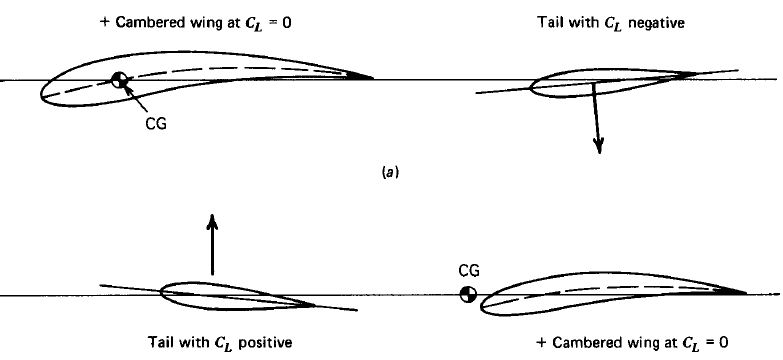
\includegraphics[scale=0.7]{20.JPG}
    \caption{Configurations avec deux surfaces portantes}
    \label{20}
\end{figure}

\subsection{Moment de tangage (pitching moment)}

Il y a quatre contributions principales au tangage (pitch) :
\begin{itemize}
    \item Les ailes
    \item Le fuselage et les nacelles
    \item L'empennage
    \item La propulsion
\end{itemize}

 \begin{figure}[h!]
     \centering
     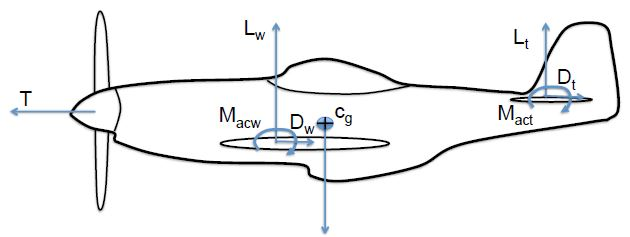
\includegraphics[scale=0.7]{21.JPG}
     \caption{Moment de tangage pour une configuration conventionnelle}
     \label{21}
 \end{figure}

\subsubsection{Contribution de l'aile principal}

\begin{figure}[h!]
    \centering
    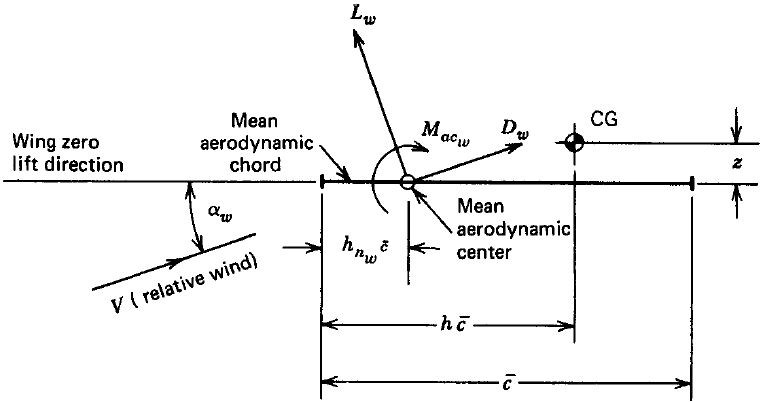
\includegraphics[scale=0.7]{22.JPG}
    \caption{Système de force et moment sur l'aile}
    \label{22}
\end{figure}

Le centre aérodynamique de l'aile (foyer) est défini comme le point autour duquel le moment des forces aérodynamiques et indépendante de l'incidence (et donc de la portance). On peut obtenir le moment autour du centre de gravité de l'avion avec les notations définies figure \ref{22} et $\bar{c}$ \textit{la corde aérodynamique moyenne} de l'aile définie par 
\begin{eqnarray}
\bar{c}=\frac{1}{S}\int_{-b/2}^{b/2}c^2dy
\end{eqnarray}

On obtient
\begin{eqnarray}
M_w = M_{ac_w}+(L_w cos\alpha_w + D_w sin \alpha_w)(h-h_{n_w})\bar{c}+(L_wsin\alpha_w-D_wcos\alpha_w)z
\end{eqnarray}

En non-dimensionnalisant par $\frac{1}{2}\rho V^2\bar{c} S$ et en supposant $\alpha <<1$ (angle d'incidence)

\begin{eqnarray}
C_{m_w}=C_{m_{acw}}+(C_{L_w}+C_{D_w}\alpha_w)(h-h_{n_w})+(C_{L_w}\alpha_w-C_{D_w})z/\bar{c}
\end{eqnarray}

Dans la plupart des cas, $z<<\bar{c}$ et la contribution de la trainée peut être négligée. On obtient finalement
\begin{eqnarray}
C_{m_w}&=C_{m_{ac_w}}+C_{L_w}(h-h_{n_w})\\
 &=C_{m_{ac_w}}+a_w\alpha_w(h-h_{n_w})
\end{eqnarray}

avec $a_w$ la pente de la courbe de portance de l'aile ($a_w=C_{L_{\alpha_w}}$).

\subsubsection{Contribution du fuselage et de la nacelle}

L'équation du moment de tangage de la combinaison aile/fuselage/nacelles prend la même forme que pour l'aile seule mais avec des valeurs différentes des paramètres :
\begin{eqnarray}
C_{m_{wb}} &= C_{m_{ac_{wb}}}+C_{L_{wb}}(h-h_{n_{wb}})\\
&= C_{m_{ac_{wb}}}+a_{wb}\alpha_{wb}(h-h_{n_{wb}})\\
\end{eqnarray}
où $a_wb$ est la pente de la courbe de portance de la combinaison aile/fuselage/nacelles.

\subsubsection{Contribution de l'empennage}

Les efforts aérodynamiques sur l'empennage s'expriment exactement de la même manière que ceux de l'aile principale, à ceci près que les interférences dues à la présence de l'aile principale doivent être prises en compte.

\begin{figure}[h!]
    \centering
    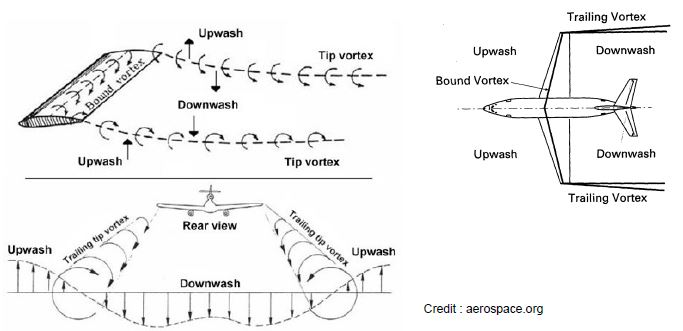
\includegraphics[scale=0.7]{23.JPG}
    \caption{Schéma de l'écoulement de l'air sur une aile d'avion}
    \label{23}
\end{figure}

\begin{figure}[h!]
    \centering
    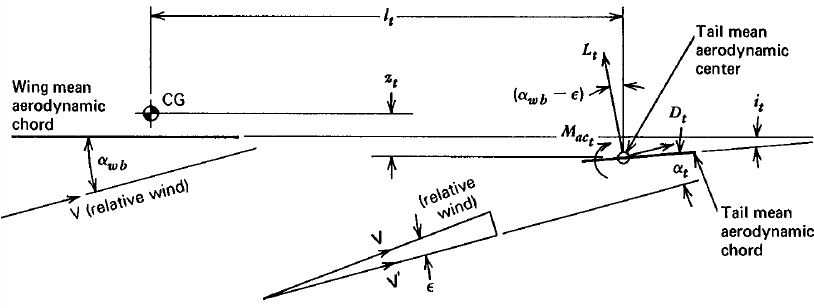
\includegraphics[scale=0.7]{24.JPG}
    \caption{Système de forces et moment sur l'empennage}
    \label{24}
\end{figure}

D'après le schéma de la figure \ref{24}, on obtient l'expression suivante pour le moment de tangage produit par l'empennage :
\begin{eqnarray}
M_t=M_{ac_t}-l_t[L_tcos(\alpha_{wb}-\epsilon)+D_tsin(\alpha_{wb}-\epsilon)]-z_t[(L_tsin(\alpha_{wb}-\epsilon)-D_tcos(\alpha_{wb}-\epsilon)]
\end{eqnarray}

où $L_t$ et $D_t$ sont respectivement portance et traînée -c'est-à-dire composantes perpendiculaires et parallèles au vent effectif $V'$ de la force aérodynamique - de l'empennage. 

\textbf{Hypothèses :}
\begin{itemize}
    \item Petits angles
    \item $z_t<<l_t$
    \item $D_t<<L_t$
    \item $M_{act}$ small
\end{itemize}

En définissant le coefficient de portance de l'empennage comme
\begin{eqnarray}
C_{L_t}=\dfrac{L_t}{\frac{1}{2}\rho V^2 S_t}
\end{eqnarray}

on obtient en adimensionnalisant à nouveau par $\frac{1}{2}\rho V^2\bar{c}S$

\begin{eqnarray}
C_{m_t} = -\dfrac{l_tS_t}{\bar{c} S}C_{L_t}
\end{eqnarray}

Le rapport $l_tS_t/\bar{c}S$ est un rapport de volumes caractéristique de la géométrie de l'avion, que l'on appelle communément "rapport de volumes de l'empennage horizontal" et que l'on note $V_H$, de sorte qu'avec cette notation, on a
\begin{eqnarray}
C_{m_t}=-V_HC_{L_t}
\end{eqnarray}

Le centre de gravité d’un avion pouvant bouger en fonction du chargement et
de la consommation de carburant, il est plus commode de définir la position
de l’empennage par rapport au foyer de la combinaison aile/fuselage/nacelles
plutôt que par rapport au centre de gravité.

On note $\bar{l_t}$ la distance le long de la direction de portance nulle de l'aile/fuselage entre le foyer de l'empennage et le foyer de l'aile, on a
\begin{eqnarray}
\bar{l_t}=l_t+(h-h_{n_{wb}})\bar{c}\\
\bar{V}_H=\dfrac{\bar{l_t}S_t}{\bar{c}S}=V_H+(h-h_{n_{wb}})\dfrac{S_t}{S}\\
C_{m_t}=-\bar{V}_HC_{L_t}+(h-h_{n_{wb}})\dfrac{S_t}{S}C_{L_t}
\end{eqnarray}

\subsubsection{Contribution du système de propulsion}

Le système de propulsion fournit deux contributions au moment de tangage
de l’avion : la contribution directe du moment des forces propulsives, et une
contribution indirecte par l’interférence entre le soufflee ou le jet propulsif et la
cellule (aile/fuselages/empennage). En supposant que les effets indirects sont intégrés dans les coefficients aérodynamiques des éléments de la cellule, il reste la contribution directe que l'on notera $C_{m_p}$.

\begin{eqnarray}
C_{m_p}=C_{m_pd}+\cancel{C_{m_pi}}
\end{eqnarray}

\subsection{Point neutre manche fixe}

En rassemblant l'ensemble des contributions au moment de tangage, on obtient
\begin{eqnarray}
C_m=C_{m_{ac_{wb}}}+C_{L_{wb}}(h-h_{n_{wb}})-\bar{V}_HC_{L_t}+(h-h_{n_{wb}})\dfrac{S_t}{S}C_{L_t}+C_{m_p}
\end{eqnarray}

Cette expression se simplifie en remarquant que
\begin{eqnarray}
C_{L_{wb}}+\dfrac{S_t}{S}C_{L_{wb}}=\dfrac{L_{wb}+L_t}{\frac{1}{2}\rho V^2\bar{c}S}=C_L
\end{eqnarray}

n'est rien d'autre que le coefficient de portance global, pour donner
\begin{eqnarray}
C_m=C_{m_{ac_{wb}}}+C_L(h-h_{n_{wb}})-\bar{V}_HC_{L_t}+C_{m_p}
\end{eqnarray}

On obtient alors la raideur en tangage en dérivant par rapport à l'angle d'incidence $\alpha$.
\begin{eqnarray}
C_{m_\alpha}=C_{L_\alpha}(h-h_{n_{wb}})-\bar{V}_H\dfrac{\partial C_{L_t}}{\partial \alpha}+\dfrac{\partial C_{m_p}}{\partial \alpha}
\end{eqnarray}

Le point pour lequel la raideur en tangage s'annule, prend un sens particulier puisqu'il définit la frontière entre centrages stables et instables. On lui donne le nom de \textit{point neutre}.
\begin{eqnarray}
h_n = h_{n_{wb}}+\dfrac{1}{C_{L_\alpha}}\left[\bar{V}_H\dfrac{\partial C_{L_t}}{\partial\alpha}-\dfrac{\partial C_{m_p}}{\partial\alpha}\right]
\end{eqnarray}

En utilisant cette définition, la raideur en tangage s'exprime simplement comme
\begin{eqnarray}
C_{m_\alpha}=C_{L_\alpha}(h-h_n)
\end{eqnarray}

\section{Guidage et stabilité statique - manche libre longitudinaux}

\subsection{Angle de gouverne}

On peut déduire à partir de l'expression finale du moment de tangage, que le point d'équilibre est obtenu pour une incidence 
\begin{eqnarray}
\alpha=\dfrac{C_{m_0}}{a(h_n-h)}
\end{eqnarray}

Il est donc possible de faire varier l'état d'équilibre en en faisant varier le centrage (la marge statique). En outre, le désavantage de faire varier la marge statique est que le point d'équilibre varie également. La marge statique diminuant, l'incidence augmente, et donc on se rapproche du décrochage.

Pour ces raisons, on préfère contrôler l'incidence de l'avion par une déformation de sa géométrie qui modifie $C_{m_0}$ en modifiant le moins possible la marge statique. 

La solution est d'ajouter un volet mobile dans l'empennage appelé \textit{gouverne de profondeur}, qui modifie la cambrure et par conséquent l'incidence de portance nulle (voir figure \ref{25}) :
\begin{figure}[h!]
    \centering
    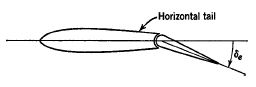
\includegraphics{25.JPG}
    \caption{Gouverne de profondeur}
    \label{25}
\end{figure}

Notant $\delta_e$ l'angle de la gouverne de profondeur, l'expression du coefficient de portance de l'empennage se modifie comme suit :
\begin{eqnarray}
C_{L_t} = a_t\alpha_t+\dfrac{\partial C_{L,t}}{\partial\delta_e}\delta_e=a_t\alpha_t+a_e\delta_e=a_t(\alpha_{wb}-i_t-\epsilon)+a_e\delta_e
\end{eqnarray}

Il s'ajoute un terme dépendant linéairement de l'angle de gouverne. 

Le coefficient de portance devient (deuxième graphe de la figure \ref{26})
\begin{eqnarray}
C_L=a\alpha+\dfrac{S_t}{S}a_e\delta_e
\end{eqnarray}

En ce qui concerne le coefficient de moment, $C_{m_\alpha}$ et donc la marge statique restent inchangés alors que $C_{m_0}$ est modifié comme suit : (premier graphe de la figure \ref{26})

\begin{eqnarray}
C_{m_0}=C_{m_{00}}+\left[\dfrac{S_t}{S}(h-h_{n_{wb}})-\bar{V}_H\right]a_e\delta_e
\end{eqnarray}

\textbf{Note :} Une déflexion positive de la gouverne déplace le point d'équilibre vers une incidence plus faible (et donc une vitesse plus élevée). (Voir figure \ref{26})
\begin{figure}[h!]
    \centering
    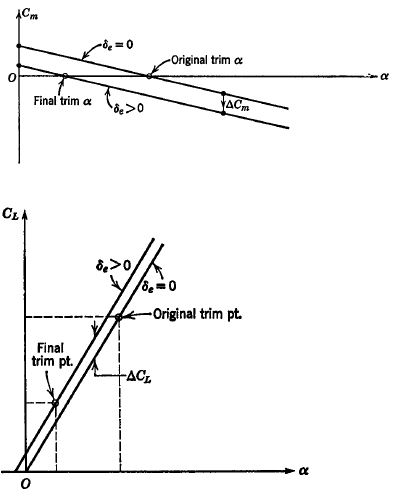
\includegraphics[scale=0.8]{26.JPG}
    \caption{Effet de la déflexion de la gouverne de profondeur sur les coefficients aérodynamiques}
    \label{26}
\end{figure}

\begin{figure}[h!]
    \centering
    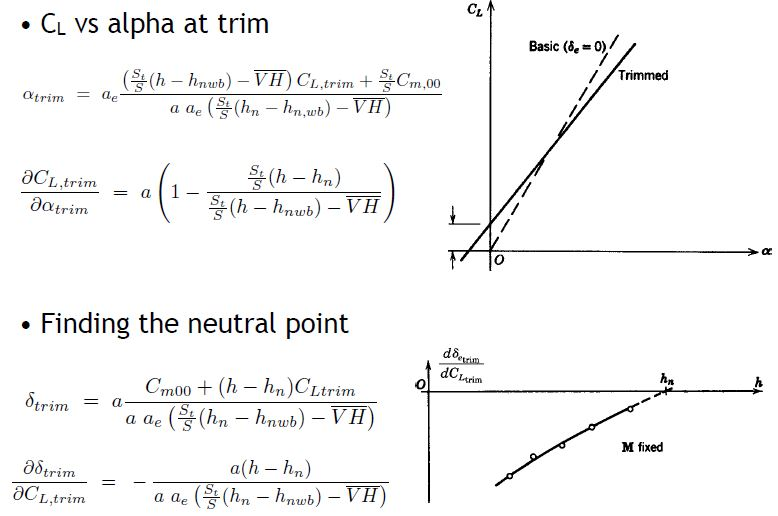
\includegraphics[scale=0.8]{27.JPG}
    \caption{Pente de la courbe de portance à l'équilibre et détermination du point neutre par essais en vol}
    \label{27}
\end{figure}
\begin{figure}[h!]
    \centering
    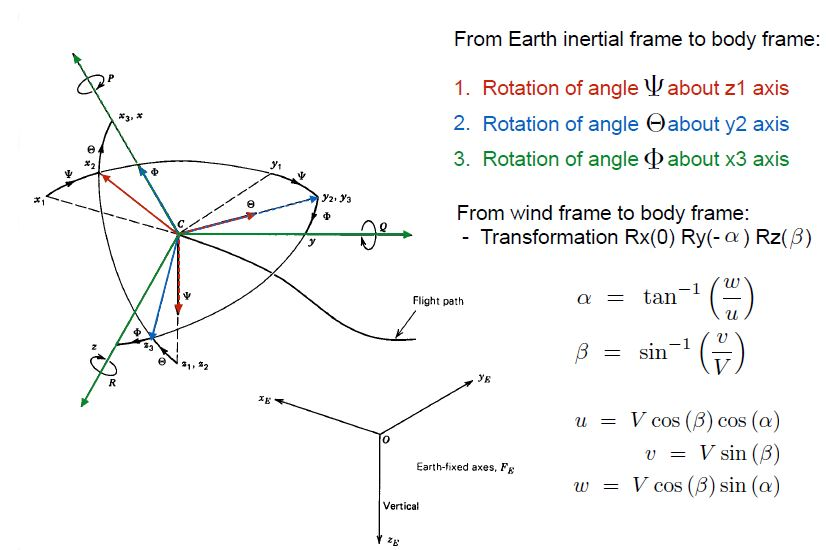
\includegraphics[scale=0.7]{28.JPG}
    \caption{Notations et repère}
    \label{28}
\end{figure}
\newpage

\section{Stabilité statique latérale}

\subsection{Définition des orientations}

\begin{figure}[h!]
    \centering
    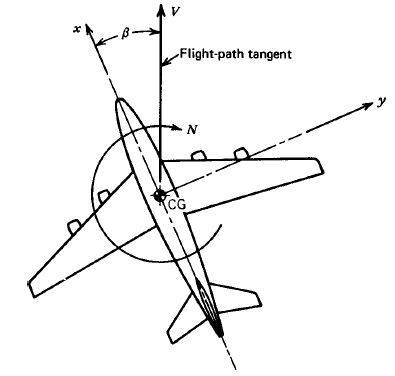
\includegraphics[scale=0.7]{29.JPG}
    \caption{Avion en dérapage}
    \label{29}
\end{figure}
\newpage

\subsection{Stabilité directionnelle et guidage}

Considérons un avion subissant une perturbation dé dérapage $\beta$ (voir figure \ref{29}). La condition de stabilité statique sera que le couple aérodynamique produit ait tendance à ramener l'avion en vol symétrique, c'est-à-dire que la raideur en lacet $\partial N/\partial B$ soit positive. Le coefficient adimensionnel de moment de lacet est
\begin{eqnarray}
C_n=\dfrac{N}{\frac{1}{2}\rho V^2 S b}\\
\dfrac{\partial C_n}{\partial\beta}>0
\end{eqnarray}

\textbf{Note :} la longeur de référence est l'envergue $b$ et non la corde $\bar{c}$.

Sa dérivée par rapport au dérapage est notée $C_{n_\beta}$ de manière analogue à la notation adoptée pour la raideur de tangage ($C_{m_\alpha}$).

On constate plusieurs effets :
\begin{itemize}
    \item effet de la dérive
    \item effet du fuselage et des ailes
    \item effet des hélices
\end{itemize}
\begin{eqnarray}
C_n=C_{n,wing}+C_{n,fuselage}+C_{n,fin}+C_{n,prop}
\end{eqnarray}

Le plus important est le rôle de la dérive (voir figure \ref{30}).

\begin{figure}[h!]
    \centering
    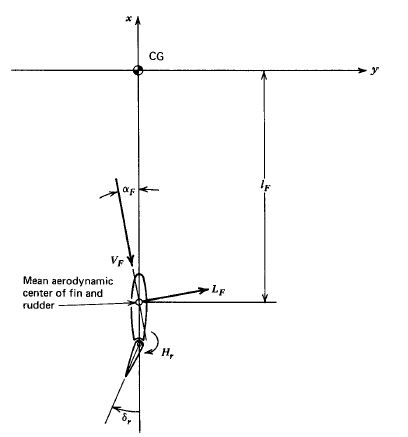
\includegraphics[scale=0.7]{30.JPG}
    \caption{Forces aérodynamiques sur la dérive}
    \label{30}
\end{figure}

On a la vitesse de l'écoulement abordant la dérive $V_F$ qui serait égale à la vitesse $V$ et à incidence $\alpha_F$ sur la dérive égale à l'opposé du dérapage $\alpha_F=-\beta$. En réalité cependant, il faut tenir compte des interférences dues au souffle des hélices, au fuselage et à l'aile. En direction, ces interférences sont représentées par une déflexion angulaire $\sigma$ semblable à la déflexion $\epsilon$ ressentie par l'empennage horizontal, à laquelle on attribue un signe positif si elle a pour effet d'augmenter l'incidence. On aura donc
\begin{eqnarray}
\alpha_F=-\beta+\sigma\\
C_{L_F}=a_F(-\beta+\sigma)+a_r\delta_r
\end{eqnarray}

avec $\delta_r$ le braquage du gouvernail, on obtient le coefficient de moment de lacet dû à la dérive
\begin{eqnarray}
C_{n_F}=-C_{L_F}\dfrac{S_F l_F}{S b}\left(\dfrac{V_F}{V}\right)^2
\end{eqnarray}

où $\dfrac{S_F l_F}{S b}$ est appelé \textit{le rapport de volumes de la dérive} et est noté $V_V$.

\begin{eqnarray}
\dfrac{\partial C_{n_F}}{\partial \beta}=V_V\left(\dfrac{V_F}{V}\right)^2a_F\left(1-\dfrac{\partial\sigma}{\partial\beta}\right)
\end{eqnarray}

On a aussi
\begin{eqnarray}
C_{n_{\delta_r}}=\dfrac{\partial C_n}{\partial \delta_r} = -a_r V_V\left(\dfrac{V_F}{V}\right)^2
\end{eqnarray}

Cette dérivée, aussi appelée \textit{puissance du gouvernail}, doit être suffisamment élevée pour maintenir un dérapage nul dans les conditions les plus défavorables d'une poussée asymétrique en virage.

Un autre indicateur utile de l’effectivité du gouvernail est l’angle de dérapage qui peut être maintenu pour un braquage de gouvernail donné. Le couple de lacet étant donné par
\begin{eqnarray}
C_n=C_{n_\beta}\beta+C_{n_{\delta_r}}\delta_r
\end{eqnarray}

$C_n=0$ à l'équilibre donc $\dfrac{\beta}{\delta_r}=-\dfrac{C_{n_{\delta_r}}}{C_{n_{\beta}}}$.

\subsection{Stabilité en roulis et guidage}

\begin{figure}[h!]
    \centering
    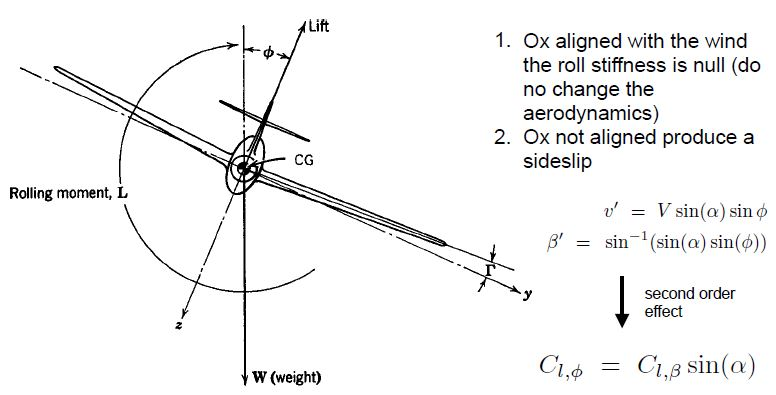
\includegraphics[scale=0.7]{31.JPG}
    \caption{Avion incliné en roulis}
    \label{31}
\end{figure}

L'effet du dièdre est représenté figure \ref{32}. On voit que la composante latérale de la vitesse ($v=Vsin\beta\approx V\beta$) fournit une contribution $v\Gamma = V\beta \Gamma$ à la vitesse normale au plan de l'aile tribord (à gauche de la figure) et un contribution opposée à la vitesse normale au plan de l'aile bâbord. Il en résulte les incréments d'incidence $\Delta\alpha=\pm \beta\Gamma$ respectivement sur les ailes tribord et bâbord, ce qui produit un couple de roulis proportionnel à $\beta\Gamma$ et donc une contribution à $C_{l_\beta}$ proportionnelle à $\Gamma$.

\begin{figure}[h!]
    \centering
    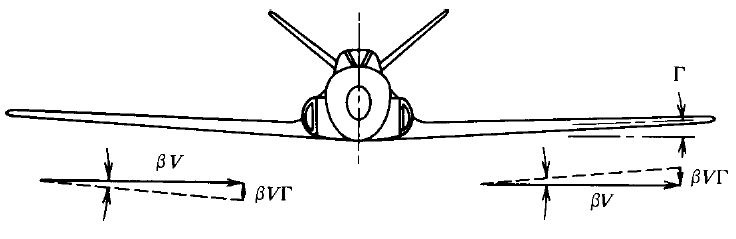
\includegraphics[scale=0.7]{32.JPG}
    \caption{Rôle du dièdre}
    \label{32}
\end{figure}

La flèche de l'aile joue également un rôle important\footnote{La flèche de l'aile est toutefois déterminée principalement en fonction de considérations autres.}. En effet, comme indiqué à la figure \ref{33}, en présence d'un dérapage, la composante de la vitesse perpendiculaire à l'axe aérodynamique de l'aile est plus élevée sur l'aile tribord que sur l'aile bâbord. Il en résulte que la portance est plus élevée également et don qu'il apparaît un couple de roulis négatif, proportionnel au coefficient de portance de l'aile et au dérapage.

\begin{figure}[h!]
    \centering
    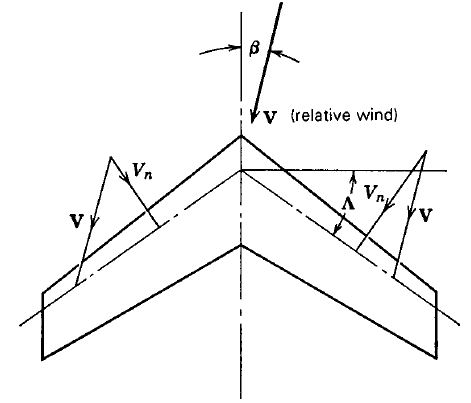
\includegraphics[scale=0.7]{33.JPG}
    \caption{Effet de la flèche sur $C_{l_\beta}$}
    \label{33}
\end{figure}

On voit (figure \ref{34}) que l'écoulement autour du fuselage induit par le dérapage a tendance à augmenter/réduire l'incidence sur l'aile tribord selon que l'aile soit en position haute ou basse et réciproquement pour l'aile bâbord. On en conclu que l'interférence aile et fuselage produit une contribution négative à $C_{l_\beta}$ pour une aile haute et positive pour une aile basse. C'est la raison pour laquelle les ailes hautes ont un dièdre moins important que les ailes basse, surtout pour les ailes en flèches, pour lesquelles on peut même observer parfois des dièdres négatifs.

\begin{figure}[h!]
    \centering
    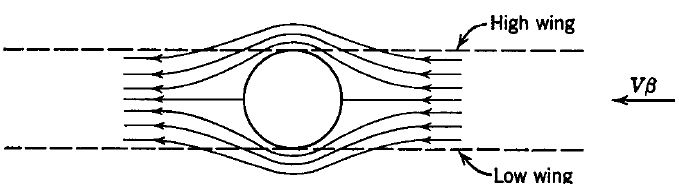
\includegraphics[scale=0.7]{34.JPG}
    \caption{Effet du fuselage sur $C_{l_\beta}$}
    \label{34}
\end{figure}

La flèche arrière augmente l'effet dièdre (le dièdre effectif); 5 degrés de flèche arrière valent environ 1 degré de dièdre.
La position haute de l'aile augmente également l'effet dièdre. Cela conduit aux valeurs de dièdre suivantes :

\begin{itemize}
    \item Aile haute,\\
sans flèche arrière : dièdre faiblement positif ou nul\\
avec flèche arrière : dièdre négatif de l'ordre de 4 à 6 degrés.
\item Aile basse,\\
sans flèche arrière : dièdre positif, valeur fréquente 4 à 5 degrés\\
avec flèche arrière : dièdre nul ou faiblement positif
\end{itemize}


Enfin, la dernière contribution importante à $C_{l_\beta}$ est celle de la dérive. La portance sur la dérive résultant d'un dérapage produit en effet un couple de roulis égal à $L_Fz_F$, où $z_F$ est la distance entre le centre aérodynamique de la dérive et l'axe $x$. Par conséquent, le coefficient de couple de roulis vaut
\begin{eqnarray}
\Delta C_l=a_F(-\beta+\sigma)\dfrac{z_FS_F}{Sb}\left(\dfrac{V_F}{V}\right)^2
\end{eqnarray}

et la contribution à $C_{l_\beta}$
\begin{eqnarray}
\Delta C_{l_\beta}=-a_F\left(1-\dfrac{\partial\sigma}{\partial \beta}\right)\dfrac{z_FS_F}{Sb}\left(\dfrac{V_F}{V}\right)^2
\end{eqnarray}

\begin{figure}[h!]
    \centering
    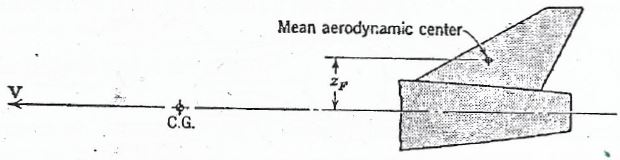
\includegraphics[scale=0.7]{35.JPG}
    \caption{Schéma de la dérive}
    \label{35}
\end{figure}

Le guidage en roulis est effectué grâce aux ailerons qui sont le plus souvent des volets mobiles de l'aile principale braqués de manière différentielle comme indiqué sur la figure \ref{36}.

\begin{figure}[h!]
    \centering
    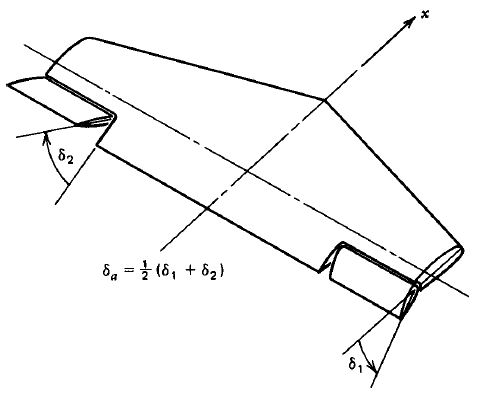
\includegraphics[scale=0.7]{36.JPG}
    \caption{Schéma de la dérive}
    \label{36}
\end{figure}


\chapter{Équations générales du mouvement}

\chapter{Dérivées de stabilité}

\begin{eqnarray}
C_x=C_T+C_L\alpha_x-C_D\\
C_z=-(C_L+C_D\alpha_x)
\end{eqnarray}

\section{Dérivées longitudinales}
\subsection{Dérivées par rapport à $\alpha$}

\paragraph{$C_{x_\alpha}$}

\begin{eqnarray}
C_{x_\alpha}=\dfrac{\partial C_x}{\partial\alpha} = \dfrac{\partial C_T}{\partial\alpha}+C_L+\alpha_x\dfrac{\partial C_L}{\partial \alpha}-\dfrac{\partial C_D}{\partial \alpha}
\end{eqnarray}

On suppose le coefficient de poussée indépendant de l'incidence et on évalue l'expression précédente à l'état d'équilibre (identifié par l'indice o, avec en particulier $\alpha_{x_0}=0$), on obtient
\begin{eqnarray}
C_{x_\alpha}=C_{L_0}-\left(\dfrac{\partial C_D}{\partial\alpha}\right)_0
\end{eqnarray}

Pour une polaire parabolique $C_D=C_{D_{par}}+kC_L^2$, l'expression devient
\begin{eqnarray}
C_{x_\alpha}=C_{L_0}-2kC_{L_0}C_{L_\alpha}
\end{eqnarray}

avec $C_{L_\alpha}$ la pente de la courbe de portance.

\paragraph{$C_{z_\alpha}$}

\begin{eqnarray}
C_{z_\alpha} = \dfrac{\partial C_z}{\partial \alpha}=-C_{L_\alpha}-C_{D_0}
\end{eqnarray}

On considère souvent $C_{D_0}$ négligeable par rapport à $C_{L_\alpha}$.

\paragraph{$C_{m_\alpha}$}

C'est la raideur en tangage discutée en détail précédemment :
\begin{eqnarray}
C_{m_\alpha}=a(h-h_n)
\end{eqnarray}

\subsection{Dérivées par rapport à u}

Elles représentent les variations des coefficients de forces et moment dues à une variation de vitesse pour une incidence et une position des commandes (profondeur et gaz) fixes.

\subsection{Dérivées par rapport à $q$}

\begin{figure}[h!]
    \centering
    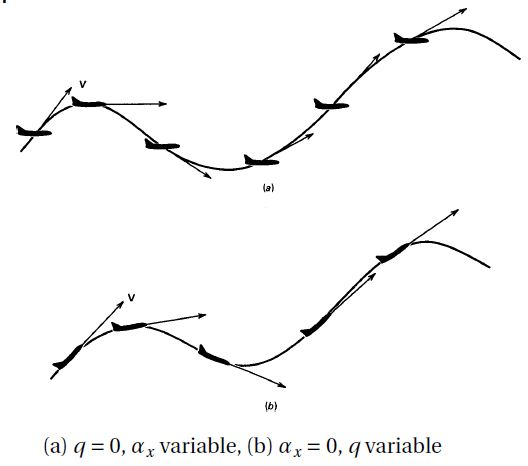
\includegraphics[scale=0.7]{37.JPG}
    \caption{Mouvements longitudinaux}
    \label{37}
\end{figure}

\subsubsection{Contribution de l'empennage}
\begin{figure}[h!]
    \centering
    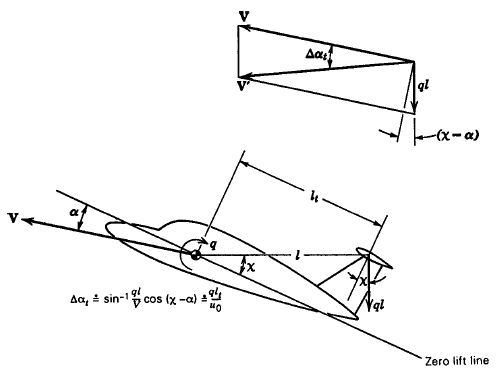
\includegraphics[scale=0.7]{38.JPG}
    \caption{Effet d'une rotation en tangage sur l'empennage}
    \label{38}
\end{figure}

L'effet principale de la rotation est d'augmenter l'incidence de l'empennage d'un angle égal à $ql_t/u_0$. En faisant l'approximation que la portance de l'empennage s'établit instantanément, cet incrément d'incidence produit donc un incrément de coefficient de portance.

\subsubsection{Contribution de l'aile}

%%%%%%%%%%%%%%%%%%%%%%%%%%%%%%%%%%%%%%%%%%%%%%%%%%%%%%%%%%%%%%%%%%%%%%%%%%%%%%%%%%%%%%%%%%%%%%%%
\newpage

\chapter{Dynamique spatiale}

\section{Les types de moteur de fusées}
\subsection{Propergol solide (solid propellant)}

Les moteurs de fusée solide sont utilisé sur des missiles air-air ou air-sol, des modèles réduits de fusée et comme boosters pour des lanceurs de satellites. Dans une fusée solide, le combustible et le comburant sont mélangés ensemble dans un propergol\footnote{Un propergol est un produit de propulsion, constitué d'un mélange de comburant et de combustible, les ergols. La réaction chimique, entre cet oxydant et ce réducteur, fournira l'énergie au moteur-fusée. Les constituants peuvent se présenter à l'état de gaz, de liquide, de solide ou de plasma.} solide qui est empaqueté dans un cylindre solide. Un trou dans le cylindre sert de chambre de combustion. Quand le combustible est enflammé, la combustion prend place à la surface du propergol. La combustion produit une grande quantité de gaz d'échappement à température et pression élevée. La quantité de gaz d'échappements qui est produite dépend de l'aire du front de flamme et les concepteurs de moteurs utilisent une variété de forme de trous pour contrôler le changement de poussée pour un moteur particulier. Les gaz chauds d'échappements passent à travers une tuyère (nozzle) qui accélère le flux. La \textbf{poussée} (thrust) est alors produite d'après la troisième loi du mouvement de Newton\footnote{The third law states that for every action (force) in nature there is an equal and opposite reaction. In other words, if object A exerts a force on object B, then object B also exerts an equal and opposite force on object A. Notice that the forces are exerted on different objects.}.

\begin{figure}[h!]
    \centering
    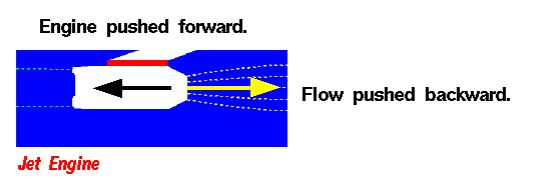
\includegraphics[scale=0.5]{39.JPG}
    \caption{Principe d'action-réaction. Troisième loi de Newton}
    \label{39}
\end{figure}

La quantité de poussée produite par la fusée dépend du design de la tuyère. La plus petite aire transversale de la tuyère est appelée \textit{col} (throat). Les gaz chauds d'échappement sont "\textit{choked}" (nombre de Mach = 1) au col, c'est à dire qu'en amont du col, la vitesse du gaz est subsonique et en aval supersonique. Cela signifie que le débit massique $\dot{m}$ est déterminé par l'aire du col. Le ratio d'aire entre le col et l'aire de sortie $A_e$ fixe la vitesse de sortie $V_e$ et la pression de sortie $p_e$. 

La pression de sortie n'est égale à la pression extérieure que dans certaines conditions. Nous devons, par conséquent, utiliser la longue version de l'équation de poussée générale pour décrire la poussée du système. Si la pression extérieure est donnée par $p_0$, l'équation de la poussée $T$ devient :

\begin{eqnarray}
T &= &\oint_{internal}pdS+P_\infty (A_i-A_e)\\
(\dot{m}_{air}+\dot{m}_{fuel})u_e-\dot{m}_{air}u_i &= &\oint_{internal}pdS+P_\infty (A_i-A_e)\\
 & \Downarrow &\text{Pour un moteur de fusée}\\
T &= &\dot{m}\cdot u_e +(p_e-p_\infty)\cdot A_e
\end{eqnarray}

Notons que le comburant est mélangé au combustible, les fusées solides peuvent donc générer de la poussée dans le vide (espace), où il n'y a pas de source d'oxygène. 

Notons également que l'équation ci-dessus fonctionne aussi bien pour du propergol solide que liquide. 

\begin{figure}[h!]
    \centering
    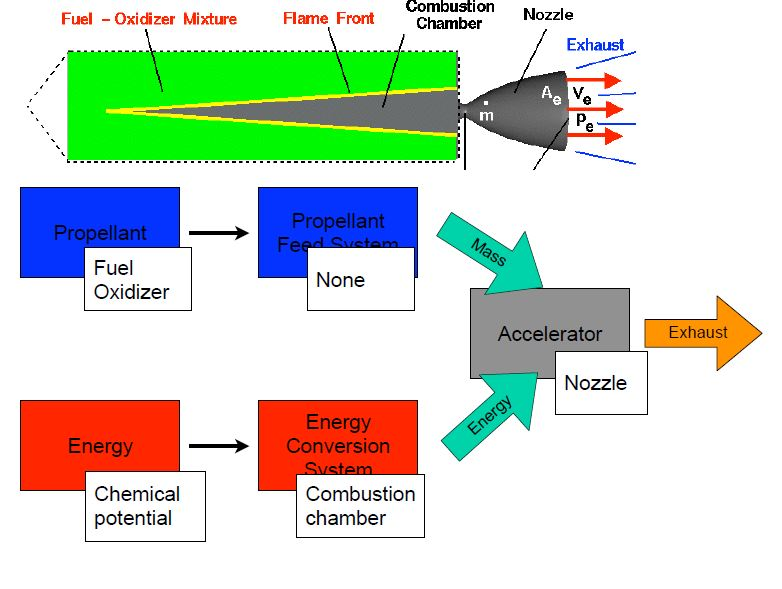
\includegraphics[scale=0.7]{40.JPG}
    \caption{Moteur de fusée à propergol solide}
    \label{40}
\end{figure}

\subsection{Propergol liquide}

Les moteurs de fusée liquide sont utilisés sur la navette spatiale pour placer des humains en orbite, sur beaucoup fusées sans humains pour placer des satellites en orbite et sur certains avions de recherches durant la deuxième guerre mondiale. Dans une fusée à propergol liquide, le combustible et le comburant stockés sont pompés dans une chambre de combustion où ils sont mélangés et brûlé. Cette combustion produit une quantité importante de gaz d'échappement à haute température et pression.

Notons que la suite du moteur à propergol liquide est exactement le même que celui à propergol solide.

\begin{figure}[h!]
    \centering
    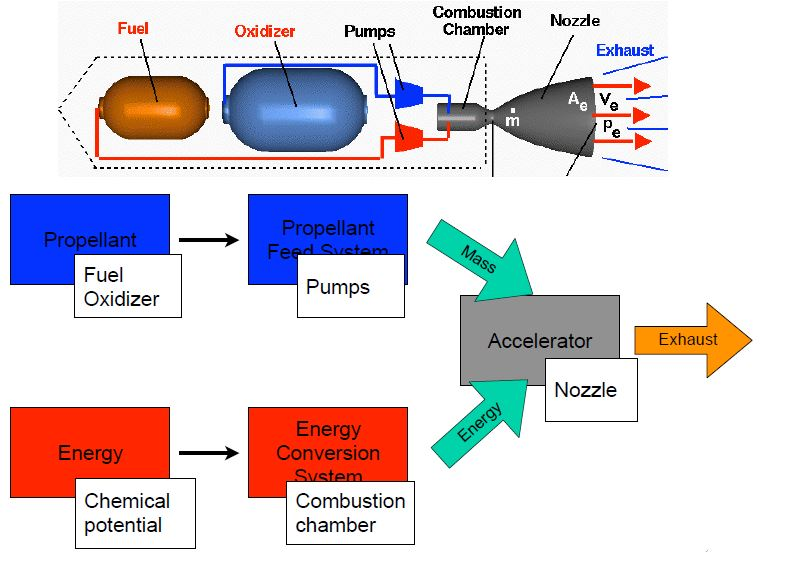
\includegraphics[scale=0.7]{41.JPG}
    \caption{Moteur de fusée à propergol solide}
    \label{41}
\end{figure}

\subsection{Système de propulsion chimique}

La propulsion chimique est une propulsion au cours de laquelle la poussée est fournie pas le produit d'une réaction chimique, la plupart du temps par combustion (ou oxydation) d'un carburant. Une réaction chimique combine deux ou plus de sortes de produits chimiques et produit différents produits chimiques. Une réaction couramment utilisée est une réaction qui combine du di-hydrogène et du di-oxygène pour faire de l'eau (figure \ref{43}).

\begin{figure}[h!]
    \centering
    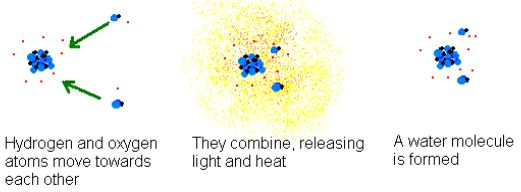
\includegraphics[scale=0.7]{43.JPG}
    \caption{Réaction chimique di-hydrogène et di-oxygène.}
    \label{43}
\end{figure}

Généralement, la réaction produit aussi de la chaleur qui va chauffer le produit. Lorsqu'un produit est chauffé, il se dilate et va être éjecté de la tuyère avec une certaine énergie cinétique. C'est ce qui produit la poussée.

La réaction chimique qui se produit dans la chambre de combustion est :
\begin{eqnarray}
O_2+2H_2~\rightarrow~2H_2O
\end{eqnarray}

\section{Fluide compressible dans une tuyère}

\begin{eqnarray}
\dfrac{dA}{A} &= &(M^2-1)\dfrac{du}{u}\\
\dfrac{T_0}{T_1} &= &\left(1+\dfrac{\gamma-1}{2}M^2\right)\\
\dfrac{p_0}{p_1} &= &\left(\dfrac{T_0}{T_1}\right)^{\frac{\gamma}{\gamma-1}}=\left(\dfrac{\rho_0}{\rho_1}\right)^\gamma\\
\dot{m} &= &\left(\dfrac{2}{\gamma+1}\right)^{\dfrac{\gamma+1}{2(\gamma-1)}}\sqrt{\dfrac{\gamma}{RT_0}}p_0 A_t\\
\dfrac{A_e}{A_t} &= &\dfrac{\sqrt{\gamma\left(\dfrac{2}{\gamma+1}\right)^{\dfrac{\gamma+1}{\gamma-1}}}}{\sqrt{\dfrac{2\gamma}{\gamma-1}\left(\left(\dfrac{p_e}{p_0}\right)^{\dfrac{2}{\gamma}}-\left(\dfrac{p_e}{p_0}\right)^{\dfrac{\gamma+1}{\gamma}}\right)}}
\end{eqnarray}

\subsection{Tuyère adaptée : les compromis}

Pour qu'une tuyère d'un moteur-fusée contribue de manière optimale à l'accélération des gaz (tuyère adaptée), il est nécessaire qu'elle soit relativement longue. Dans le cas de la fusée Ariane 5 par exemple, la tuyère du moteur Vulcain devrait, pour produire la poussée optimale, avoir une longueur de 7 mètres. Les divergents des moteurs propulsant les étages supérieurs des lanceurs doivent être particulièrement longues car la pression externe est quasi nulle. La longueur de la tuyère entraîne un allongement du lanceur et donc un alourdissement de la structure ce qui est préjudiciable aux performances globales.

\begin{itemize}
    \item Une tuyère de moteur-fusée propulsant de premier étage est amenée à fonctionner dans des conditions de pression externe très différentes : celle-ci est de 1 bar au lancement mais quasi nulle lorsque le moteur s'éteint. La géométrie de la tuyère ne peut s'adapter aux variations continues de la pression externe. Le choix effectué est sous détendre les gaz en sortie du divergent c'est-à-dire que sa pression est supérieure à celle de l'air ambiant sur la majorité du temps de fonctionnement de l'étage. Ceci permet de disposer d'une tuyère courte dont à raccourcir la masse du lanceur.
    \item Toutefois au moment de la montée en puissance du moteur-fusée avant le décollage et à l'extinction du moteur les gaz produits sont temporairement en sur-détente ce qui crée un décollement des flux pouvant endommager la tuyère au décollage et générer des poussées non symétriques au décollage comme à l'extinction.
\end{itemize}

\begin{figure}[h!]
    \centering
    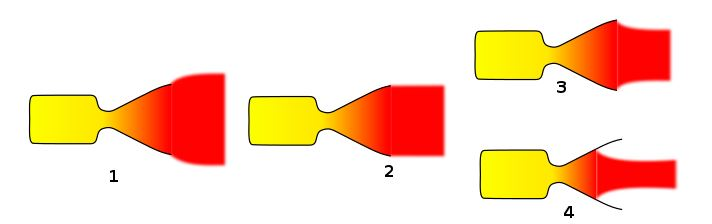
\includegraphics[scale=0.7]{44.JPG}
    \caption{Régimes de fonctionnement d'une tuyère de moteur-fusée en fonction de l'écart entre la pression des gaz en sortie du divergent et la pression extérieure ambiante. De gauche à droite :\\
1. Sous-détente des gaz en sortie de divergent : la pression ambiante est inférieure à la pression des gaz\\
2. Tuyère adaptée : égalité de la pression des gaz en sortie et de la pression ambiante (régime optimal)\\
3. Sur-détente des gaz en sortie du divergent\\
4. Sur-détente importante des gaz en sortie du divergent avec décollement du flux le long de la paroi du divergent}
    \label{44}
\end{figure}

\begin{figure}[h!]
    \centering
    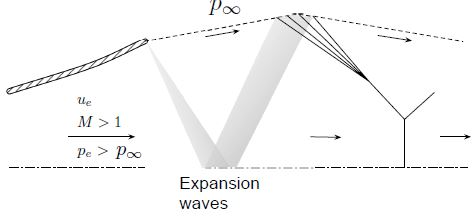
\includegraphics[scale=0.7]{45.JPG}
    \caption{Tuyère sous-détendue}
    \label{45}
\end{figure}
\begin{figure}[h!]
    \centering
    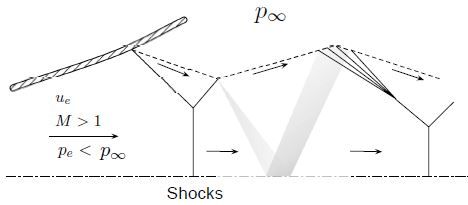
\includegraphics[scale=0.7]{46.JPG}
    \caption{Tuyère sur-détendue}
    \label{46}
\end{figure}

\subsection{Le design de la tuyère devrait être adaptée avec l'altitude}

Il y a deux types de tuyère :
\begin{itemize}
    \item Délimitée : l'expansion est imposée par la géométrie de la tuyère
    \item Libre d'expansion : l'expansion répond à la pression ambiante
\end{itemize}

\begin{figure}[h!]
    \centering
    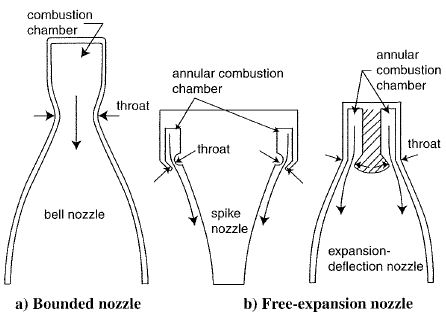
\includegraphics[scale=0.7]{47.JPG}
    \caption{Différents types de tuyères}
    \label{47}
\end{figure}

\subsubsection{Forme du divergent}

La forme du divergent doit être telle que sa paroi se confond avec la ligne de courant de l'écoulement des gaz expulsés. Ce profil se calcule généralement en résolvant les équations d'Euler en particulier en utilisant la méthode des caractéristiques. Dans le cas des tuyères utilisées dans le domaine des jets de plasma, les températures et donc les viscosités très élevées nécessitent le recours à la résolution des équations de Navier-Stokes. Le profil optimal est celui d'un cône dont le demi-angle au sommet est de 15°. Afin de raccourcir la longueur du divergent et ainsi de réduire la longueur du lanceur et donc sa masse deux solutions sont mises en œuvre :

\begin{itemize}
    \item \textit{La tuyère idéale tronquée} (TIC) est une tuyère dont le profil suit la courbe optimale mais qui est amputée de son extrémité. Dans le cas du moteur Vulcain, le fait de tronquer de 2/3 le profil idéal (longueur de 2,5 mètres au lieu de 7 mètres) entraîne une perte de poussée limitée à 3 $\%$.
    \item \textit{La tuyère optimisée à choc interne} (TOC = Thrust-Optimized Contour) est une tuyère dont le profil s'écarte de la courbe optimale ce qui permet de gagner encore 20 $\%$ sur la longueur du divergent par rapport à une tuyère de type TIC. L'angle au voisinage du col (de 20 à 50°) est supérieur à l'angle optimal ce qui permet d'accroître plus rapidement le diamètre du divergent. L'écart par rapport au profil idéal se réduit progressivement pour ne plus atteindre qu'environ 10$\degree$ à l'extrémité du divergent. La forme obtenue est dite en coquetier. Ce gain s'obtient au prix d'un écoulement du gaz plus perturbé qui peut donner lieu à des ondes de choc interne dans le divergent.
\end{itemize}

\begin{figure}[h!]
    \centering
    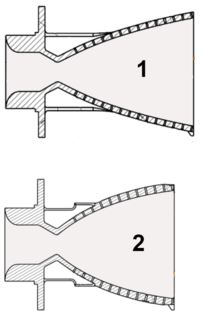
\includegraphics[scale=0.7]{48.JPG}
    \caption{Comparaison des sections de tuyère de moteur-fusée de type : 1 - TIC : Tuyère idéale tronquée 2 - TOC Tuyère en coquetier}
    \label{48}
\end{figure}

Une autre manière de réduire la longueur du divergent est de multiplier le nombre de tuyères associés à une unique chambre de combustion. Plusieurs moteurs-fusées à ergols liquides soviétiques/russes utilisent cette technique dont le RD-171 qui dispose de 4 tuyères. Le débit de chaque tuyère étant le quart du débit total, la taille du col est réduite et en conséquence le diamètre et la longueur du divergent. Le gain en longueur est évalué à 30 $\%$ avec en contrepartie une plus grande complexité et sans doute une masse plus importante qu'une configuration mono tuyère.

\subsubsection{Tuyère à divergent extensible}

Les moteurs-fusées d'étage supérieur nécessitent des tuyères très longues car elles fonctionnent dans le vide. Pour limiter la masse structurelle qu'imposerait une tuyère très longue certains moteurs comme le RL-10 B-2 qui propulse le second étage du lanceur Delta IV, comportent un divergent extensible qui n'est complètement déployé que lorsque l'étage inférieur a été largué.

\begin{figure}[h!]
    \centering
    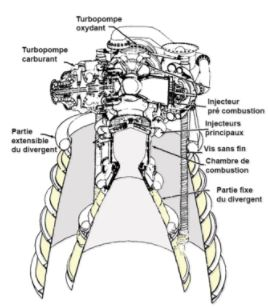
\includegraphics[scale=1]{49.JPG}
    \caption{Schéma du RL-10 à divergent extensible.}
    \label{49}
\end{figure}

\subsubsection{Tuyère à écoulement externe/corps central (par ex aerospike)}

La tuyère aerospike est un type de tuyère expérimenté sur les moteurs-fusées à ergols liquides qui permet d'optimiser l'efficacité de la propulsion dans une large gamme d'altitudes ( = de pression atmosphérique). Un moteur-fusée équipé d'une tuyère aerospike utilise 25 à 30 $\%$ de carburant en moins à basse altitude là où les lanceurs ont besoin des poussées les plus importantes. Ce type de tuyère fait l'objet d'études depuis le début de l'ère spatiale mais sa mise au point se heurte au problème de refroidissement de la rampe qui canalise le jet de gaz. Seuls des prototypes de ce type de tuyère ont été construits. La tuyère aerospike joue notamment un rôle central dans l’architecture des projets de lanceurs orbitaux monoétages (SSTO) dont les moteurs doivent fonctionner dans une gamme de pression allant de la pression au niveau de la mer jusqu'au vide.

\begin{figure}[h!]
    \centering
    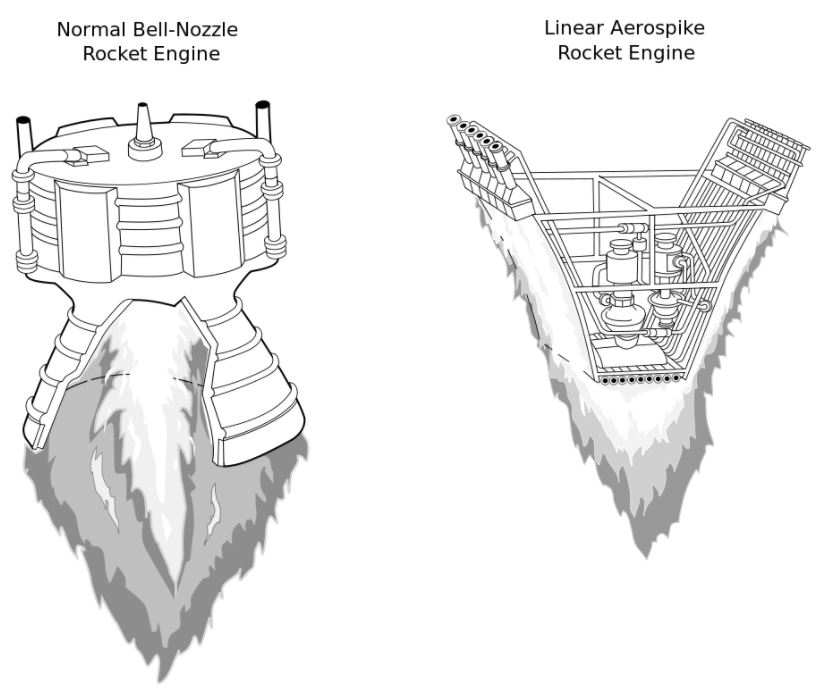
\includegraphics[scale=0.5]{50.JPG}
    \caption{Schéma comparant deux moteurs-fusées mettant en œuvre d'une part une tuyère classique et d'autre part une tuyère de type Aerospike.}
    \label{50}
\end{figure}

\paragraph{Principe de la tuyère aérospike}

Les moteurs-fusées classiques ne donnent le meilleur de leur performance qu'à une altitude donnée. Le rendement du moteur-fusée est en effet déterminé par la forme de la tuyère qui est fixe. Dans celle-ci les gaz brûles se détendent et transforment leur énergie thermique en énergie cinétique à l'origine de la poussée qui propulse la fusée. La forme et la longueur de la tuyère déterminent la pression de sortie des gaz brûlés ; or pour que le moteur fonctionne à son meilleur rendement, il est nécessaire que cette pression de sortie soit égale à la pression atmosphérique externe. Pour optimiser la poussée du moteur il serait nécessaire que la pression des gaz en sortie diminue progressivement (allongement de la tuyère et évolution de sa forme) au fur et à mesure que la fusée s'élève et que la pression atmosphérique ambiante diminue.

La tuyère de type aerospike apporte une solution au problème de l'adaptation de la tuyère à la pression ambiante. Avec ce type de tuyère les gaz en sortie de la chambre de combustion sont éjectés, non pas dans une tuyère aux parois fixes mais le long d'une structure fixe (la rampe). Les gaz se détendent en étant canalisés d'une part par la rampe d'autre part par la masse d'air ambiante. Par cette méthode la pression des gaz éjectés s'adapte automatiquement à la pression ambiante. Différentes formes de tuyère aerospike ont été étudiées : linéaire, annulaire... La rampe peut se terminer par une pointe ou être tronquée en expulsant des gaz formant une zone de surpression la prolongeant. Les gaz peuvent être produits par plusieurs chambres de combustion placés en couronne autour de la rampe centrale ou par une chambre unique qui les expulse à travers une fente annulaire.

L'idée derrière la conception de la tuyère aerospike est qu'à basse altitude, la pression ambiante comprime le jet de gaz contre la rampe centrale. La recirculation dans la zone de base de la rampe permet d'élever la pression ambiante à proximité. Comme la pression sur le dessus du moteur est ambiante, cela signifie que la base ne donne aucune poussée générale (mais cela signifie aussi que cette partie de la tuyère ne perd pas de poussée en formant un vide partiel, donc la partie de base de la tuyère peut être ignorée à basse altitude).

Lorsque la fusée prend de l'altitude, la pression d'air qui comprime le jet de gaz contre la rampe diminue, mais la pression au-dessus du moteur diminue en même temps et ce n'est donc pas nuisible. En outre, bien que la pression de base chute, la zone de redirection maintient la pression sur la base jusqu'à une fraction de 1 bar, une pression qui n'est pas équilibrée par le vide à proximité sur le dessus du moteur; cette différence de pression donne une poussée supplémentaire en altitude, créant un effet de compensation d'altitude. Cela produit le même effet que celui d'une cloche qui devient plus grande à mesure que la pression baisse, fournissant une compensation d'altitude.

Les inconvénients des moteurs aerospike sont le poids supplémentaire de la rampe centrale mais surtout la nécessité de refroidir suffisamment la rampe directement frappée par les jets de gaz en sortie de la chambre de combustion. En outre, la plus grande surface refroidie peut réduire les performances en deçà des niveaux théoriques en réduisant la pression contre la tuyère. De plus, les moteurs aerospike ont un rendement faible lorsque la vitesse est peu élevée (Mach 1-3) car le flux d'air autour du véhicule n'exerce pas assez de pression, ce qui diminue la poussée.

\subsection{Impulsion spécifique et vitesse d'échappement équivalente}

Reprenons l'équation de la poussée et divisons la par $\dot{m}$ :
\begin{eqnarray}
\dfrac{T}{\dot{m}} = u_e+(p_e-p_0)\dfrac{A_e}{\dot{m}}
\end{eqnarray}

Nous définissons une nouvelle vitesse dire \textit{vitesse équivalent} $c$ :
\begin{eqnarray}
c = u_e+(p_e-p_0)\dfrac{A_e}{\dot{m}}
\end{eqnarray}

de sorte que
\begin{eqnarray}
T = \dot{m} \cdot c
\end{eqnarray}

\textbf{L'impulsion totale ($I$)} d'une fusée est définie comme la moyenne de la poussée multipliée par le temps total du tir (firing). Définissons le temps total comme $\Delta t$ :

\begin{eqnarray}
I=T\cdot\Delta t
\end{eqnarray}

Puisque la poussée peut changer avec le temps, nous pouvons aussi définir une équation intégrale pour l'impulsion totale. 
\begin{eqnarray}
I &= &\int T dt\\
I &= &\int(\dot{m} c)dt
\end{eqnarray}

On peut donc intégrer cette équation :
\begin{eqnarray}
I = m\cdot c
\end{eqnarray}

où $m$ est la masse totale de propergol. Nous pouvons diviser cette équation par le poids du porpergol pour définir \textbf{l'impulsion spécifique}. Le mot "spécifique" signifie simplement "divisé par le poids". L'impulsion spécifique $I_{sp}$ est donnée par :
\begin{eqnarray}
I_{sp}  = \dfrac{c}{g_0}
\end{eqnarray}

avec $g_0$, l'accélération gravitationnelle au niveau de la mer. Maintenant, nous pouvons l'exprimer en fonction de la poussée :
\begin{eqnarray}
I_{sp} = \dfrac{T}{\dot{m} g_0}~~[sec]
\end{eqnarray}

Pourquoi sommes-nous intéressé par l'impulsion spécifique ? 

Premièrement, cela nous donne une manière rapide de déterminer la poussée d'une fusée, si nous connaissons le débit massique à travers la tuyère. 

Deuxièmement, c'est une indication sur le rendement du moteur. Deux moteurs différents de fusée ont une valeur de l'impulsion spécifique différente. Le moteur avec la plus grande impulsion spécifique a un meilleur rendement parce qu'il produit plus de poussée pour une même quantité de propergol. 

Troisièmement, cela simplifie les analyses mathématiques de la thermodynamique des fusées. L'unité de l'impulsion spécifique est la même, que nous utilisions les unités métriques ou anglosaxones.

Quatrièmement, cela nous donne une manière simple de dimensionner un moteur durant une étude préliminaire. Le résultat de notre analyse thermodynamique a une certaine valeur d'impulsion spécifique. Le poids de la fusée va définir une valeur de la poussée. En divisant la poussée requise par l'impulsion spécifique, nous saurons quel débit massique de porpergol le moteur va produire et donc sa taille.

\begin{figure}[h!]
    \centering
    \includegraphics{51.JPG}
    \caption{Impulsion spécifique en fonction du nombre de Mach : Quelques valeurs}
    \label{51}
\end{figure}


\section{La poussée revisitée}

\begin{eqnarray}
x_G &= &\dfrac{\sum m_i x_i}{M}\\
M x_G &= &\sum m_i x_i\\
\dfrac{dM}{dt}x_G + M\dfrac{dx_G}{dt} &= &\sum m\dfrac{x_i}{dt}
\end{eqnarray}

avec $\dfrac{dM}{dt} = -\dot{m}$, $\dfrac{dx_G}{dt} = u_G$ et $\dfrac{dx_i}{dt} = u_i$.

\begin{eqnarray}
q(t) &= &\sum m_i(u_i+u_s) = M(u_G+u_s)-\dot{m}x_G\\
q(t+dt) &= &(M+dM)(V+dV)-(\dot{m}+d\dot{m})(x_G+dx_G)-dM(u_s-u_e)\\
q(t+dt) &= &(M-\dot{m}dt)(V+dV)-(\dot{m}+\dfrac{\dot{m}}{dt})(x_G+u_Gdt)+\dot{m}dt(u_s-u_e)\\
dq =\dfrac{dq}{dt}dt &= & \cancel{MV}+MdV-\dot{m}dtV-\dot{m}dt dV - \dot{m}x_G -\dfrac{d\dot{m}}{dt}dtdx_G-\dot{m}u_G dt + \dot{m}(u_s-u_e)dt -\cancel{MV}+\dot{m}_G\\
 &= &MdV-2\dot{m}u_Gdt-\dfrac{d\dot{m}}{dt}x_e dt-\dot{m}u_e dt
\end{eqnarray}

Et nous trouvons l'équation de RANKINE :
\begin{eqnarray}
\boxed{\dfrac{dq}{dt}=M\dfrac{dV}{dt}-2\dot{m}u_G-\dfrac{d\dot{m}}{dt}x_G-\dot{m}u_e=\sum F_{ext}}
\end{eqnarray}

Simplifications :\\
\begin{itemize}
    \item $\dot{m}$ est la plupart du temps constant : $\dfrac{d\dot{m}}{dt}=0$
    \item $u_e \approx 2000...4000~~[m/s]$
    \item $u_G=O,O5~~[m/s]$
    \item $\dot{m}u_e >> 2\dot{m}u_G$
    \item $\Rightarrow \boxed{M\dfrac{dV}{dt}=\dot{m}u_e+\sum F_{ext}}$
\end{itemize}

avec $F_{ext}$ comprenant la garvité, les forces aérodynamiques (Drag($\rho,V)$, T:($p_e-p_\infty)A$).

\begin{eqnarray}
M\dfrac{dV}{dt}=\dot{m}u_e + (p_e-p_\infty) A_e - D-M_{g_x}
\end{eqnarray}

\begin{eqnarray}
\boxed{M\dfrac{dV}{dt}=T-D-M_{g_x}}
\end{eqnarray}

\subsection{Equation de la fusée}

\subsubsection{Cas 1 : pas de traînée, pas de gravité (equation de la fusée idéale)}

Equation de Tsiolkovski :

\begin{eqnarray}
\boxed{V-V_0=c ln\left(\dfrac{M_0}{M_{final}}\right)=I_{sp} g_0 ln\left(\dfrac{M_0}{M_{final}}\right)}
\end{eqnarray}

\subsubsection{Cas 2 : Pas de traînée mais gravité}

\begin{eqnarray}
\boxed{V-V_0=c ln\left(\dfrac{M_0}{M_{final}}\right) - \int_{T_0}^{t}g_x dt}
\end{eqnarray}

avec $\int_{T_0}^{t}g_x dt$ la perte due à la gravité qui dépend de la trajectoire.

\subsection{Mouvement vertical dans un champ gravitationnel}

Hypothèses :

\begin{itemize}
    \item $g_x=g$
    \item Poussée constante
    \item Débit massique constant
\end{itemize}

Définitions : 

\begin{itemize}
    \item Rapport massique : $\mu=\dfrac{M_0}{M}$
    \item Rapport poussée-poids = $R=\dfrac{T}{M_0 g_0}$
\end{itemize}

\begin{eqnarray}
\Delta V = V-V_0 &= & c ln\left(\dfrac{M_0}{M}\right)-g t_{final}
\end{eqnarray}

On considère $T=cste=\dot{m}c$\\
$dt=\dfrac{-c}{T}dM$\\
$t_{final}=\dfrac{c}{T}(M_0-M_{fuel})$
\begin{eqnarray}
\Delta V &= &c\left(ln(\mu)-\dfrac{1}{R}\left(1-\dfrac{1}{\mu}\right)\right)\\
 &\downarrow &\text{Pour un vol \textbf{non vertical} :}~~ \bar{g}_xt_{fin}=\int_0^{t_{fin}} g_x dt\\
\Delta V &= &c\left(ln(\mu)-\dfrac{\bar{g}_x}{gR}\left(1-\dfrac{1}{\mu}\right)\right)
\end{eqnarray}

\textbf{Notes :}
\begin{itemize}
    \item L'impulsion spécifique a une valeur : $I_{sp}\approx [200~-~400]~~[s]$
    \item Le rapport poussée-poids a une valeur : $T\approx [1.2~-~2]$\\
    Celle-ci est limitée par les contraintes des matériaux et une limite d'accélération supportable pour des humains.
    \item Le rapport de masses : $\mu_{max}\approx 12$\\
    Structure restante, réservoirs, pompes -> problèmes technologiques pour construire la structure légère et forte.
\end{itemize}

La vitesse finale peut être obtenue comme :
\begin{eqnarray}
\Delta V_{final} = \Delta V_{in}+\Delta V_{gravite} +\Delta V_{atm}+\Delta V_{???}
\end{eqnarray}

Pour atteindre une vitesse supérieure, on peut 
\begin{itemize}
    \item changer le moteur ($T~\uparrow$) mais le moteur sera plus gros ($\mu \downarrow$)
    \item Avoir une plus grande $I_{sp}$ (différent type de propergol) but $\mu \downarrow$
\end{itemize}

On démontre qu'une fusée composée d'un seul étage ne pourrait placer en orbite une charge utile même si elle utilise les ergols les plus performants et que son indice constructif est particulièrement faible.

Pour optimiser ses performances, une fusée doit donc être multiétages : chaque étage est doté de son ou de ses propres moteurs-fusées et est largué lorsque le carburant est épuisé. Le moteur de l'étage suivant est alors allumé.

Le premier étage des lanceurs modernes est souvent constitué d'un étage principal flanqué d'étages appelés accélérateurs dont le rôle est de fournir une poussée additionnelle durant les premières minutes du vol. Ces accélérateurs qui sont généralement à poudre peuvent avoir une poussée supérieure au premier étage (Ariane 5) proprement dit mais sont largués longtemps avant que le premier étage ait épuisé son carburant.

Traditionnellement les lanceurs spatiaux ont 3 étages (Ariane 1 et 4, Saturn V) ou 2 étages + accélérateurs accolés au 1er étage (Ariane 5…). Le dernier étage propulsif communique la part la plus importante de la vitesse horizontale au satellite. Pour augmenter ses performances, on choisit souvent une propulsion cryogénique. Cet étage dans les lanceurs les plus sophistiqués peut être éteint et rallumé plusieurs fois ce qui donne plus de souplesse pour mettre en place les charges utiles sur leurs orbites.

\begin{figure}[h!]
    \centering
    \includegraphics[scale=0.7]{52.JPG}
    \caption{Limite des fusées mono-étagées}
    \label{52}
\end{figure}


\subsection{Trajectoire d'un vol}

Objectif :
\begin{itemize}
    \item Minimiser les contraintes sur le lanceur $\dfrac{\rho V^2 S}{2}$
    \item Minimiser les pertes dues à la gravité
\end{itemize}

Il y a deux phases lors d'un vol :
\begin{itemize}
    \item \textit{La phase verticale} : peu de contraintes mais beaucoup de pertes gravitationnelles
    \item \textit{La trajectoire inclinée} : plus de contraines structurales mais moins de pertes gravitationnelles
\end{itemize}

\subsection{Fusées multi-étagées}

\begin{figure}[h!]
    \centering
    \includegraphics[scale=0.7]{53}
    \caption{Fusée multi-étage}
    \label{53}
\end{figure}

Dans le multi-étage \textbf{en série} (figure \ref{54}), il y a un petit second étage qui est placé au-dessus du premier plus grand. Le premier étage est utilisé au décollage et brûle jusqu'à épuisement de son propergol. Il est ensuite largué et le second étage est allumé. La charge utile est bien évidemment dans l'étage supérieur.

\begin{figure}[h!]
    \centering
    \includegraphics[scale=0.7]{54}
    \caption{Étages en série}
    \label{54}
\end{figure}

Dans le multi-étage \textbf{parallèle} (figure \ref{55}), il y a a de petits étages de chaque côté de l'étage central. Au lancement, tous les étages sont allumés. Lorsque le propergol dans les petits étages est consommé, ils sont largués. L'étage central continue de brûler jusque dans l'espace et contient la charge utile dans sa partie haute.

\begin{figure}[h!]
    \centering
    \includegraphics[scale=0.7]{55}
    \caption{Étages parallèles}
    \label{55}
\end{figure}

\subsubsection{Optimisation de l'étagement en série :}

Il faut minimiser le rapport de masse final : $\left(\dfrac{M_{01}}{M_{payload}}\right)_min$\\

\begin{eqnarray}
\Delta V_{tot} &= &\Delta V_{orbit}+\Delta V_{gravite} +\Delta V_{atm}\\
g(\mu_1,\mu_2,\mu_3) &= &\sum_{i=1}^N c ln(\mu)-\Delta V_{tot} = 0\\
 M_{oi} &= &M_{oi-1}-M_{prop,i-1}-M_{struct,i-1} \\
\sigma_i &= &\dfrac{M_{struct,i}}{M_{struct,i}-M_{prop,i}}\\
\mu_i &= &\dfrac{M_{o,i}}{M_{o,i}-M_{prop,i}}\\
\dfrac{M_{o,i}}{M_{o,i}-M_{p,i}-M_{s,i}} &= &\dfrac{\mu_i(1-\sigma_i)}{(1-\mu_i\sigma_i}\\
\dfrac{M_{o,i}}{M_{payload}} &= &\Pi_{i=1}^N\dfrac{\mu_i(1-\sigma_i)}{(1-\mu_i\sigma_i)}
\end{eqnarray}

On veut minimiser $\dfrac{M_{o,i}}{M_{payload}}$ par rapport à $\mu_i$. Cela revient à minimiser $ln\left(\dfrac{M_{o,i}}{M_{payload}}\right)$
\begin{eqnarray}
ln\left(\dfrac{M_{o,i}}{M_{payload}}\right) &= &\sum_{i=1}^N \left(ln(\mu_i)+ln(1-\sigma_i)-ln(1-\sigma_i\mu_i)\right)\\
F &= &\sum_{i=1}^N \left(ln(\mu_i)+ln(1-\sigma_i)-ln(1-\sigma_i\mu_i)\right) + \lambda\sum_{i=1}^N c_iln(\mu_i)-\Delta V_{tot}
\end{eqnarray}

avec $\lambda\sum_{i=1}^N c_iln(\mu_i)-\Delta V_{tot}$ les contraintes.

\[
\begin{cases}
\dfrac{\partial F}{\partial\mu_i} = \dfrac{1}{\mu_i}\left(\dfrac{-\sigma_i}{1-\mu_i\sigma_i}\right) + \lambda c_i\dfrac{1}{\mu_i}=0\\
\dfrac{\partial F}{\partial\lambda}=\sum_{i=1}{N}c_i ln(\mu_i)-\Delta V_{tot} = 0
\end{cases}
\]

\begin{figure}[h!]
    \centering
    \includegraphics[scale=0.7]{56}
    \caption{Étages parallèles}
    \label{56}
\end{figure}

\section{Manoeuvres orbitales}

\subsection{Problème de deux corps (Keplerian orbit)}

Loi de la gravité universelle pour N corps :
\begin{eqnarray}
\vec{F_i}= G m_i \sum_{i=1,j\ne 1}^N \dfrac{m_j}{(\vec{r}_j-\vec{r}_i)^3}(\vec{r}_j-\vec{r}_i)
\end{eqnarray}

avec $G=6,67259\cdot10^{-11}~~\left[\dfrac{Nm^2}{kg^2}\right]$.

\begin{eqnarray}
g = \dfrac{GM}{R^2}
\end{eqnarray}

Selon le principe d'action-réaction :
\begin{eqnarray}
\vec{F_1}=-\vec{F_2} &= &m_1m_2\dfrac{G}{\vec{r}^3}|\vec{r}|\\
\vec{F_2} &= &m_2\ddot{\vec{r_2}}=-m_1\ddot{\vec{r_1}}
\end{eqnarray}

On peut donc arriver à

\begin{eqnarray}
\vec{F_2}=\dfrac{m_1m_2}{m_1+m_2}\ddot{\vec{r}}\\
\boxed{\mu \ddot{r}+m_1m_2G\dfrac{|r|}{(r^3)}=0}
\end{eqnarray}

avec $\mu=\dfrac{m_1m_2}{m_1+m_2}\approx m_2$ car $m_1>>>m_2$

\begin{eqnarray}
\boxed{m_2\ddot{r}+Gm_1m_2\dfrac{|\vec{r}|}{(r)^3}=0}
\end{eqnarray}
\begin{eqnarray}
K = Gm_i=gR^2=9,81\cdot (6371~[km])^2
\end{eqnarray}






\end{document}